\subsection{Контрольная номер 1, базовый поток, 26.10.2015}

\begin{enumerate}
\item
Подбрасываются две симметричные монеты. Событие А — на первой монете выпал
герб, событие В — на второй монете выпал герб, событие С — монеты выпали
разными сторонами.
\begin{enumerate}
    \item[$\alpha$)] Будут ли эти события попарно независимы?
    \item[$\beta$)]  Сформулируйте определение независимости в совокупности для трех событий. Являются ли события $A$, $B$, $C$ независимыми в совокупности?
\end{enumerate}

\item
Имеются два игральных кубика:
\begin{itemize}
    \item красный со смещенным центром тяжести, так что вероятность выпадения «6»
    равняется 1/3, а оставшиеся грани имеют равные шансы на появление
    \item честный белый кубик
\end{itemize}

\begin{enumerate}
    \item[$\alpha$)] Петя случайным образом выбирает кубик и подбрасывает его. Найдите
    вероятность того, что выпадет «6».
    \item[$\beta$)]   Петя случайным образом выбирает кубик и подбрасывает его. Какова
    вероятность того, что Петя взял красный кубик, если известно, что выпала
    шестерка?
\end{enumerate}

\item
Все те же кубики. Петя играет с Васей в следующую игру: Петя выбирает кубик и
подбрасывает его. Вася подбрасывает оставшийся кубик. Выигрывает тот, у кого
выпало большее число. Если выпадает равное число очков, выигрывает тот, у кого
белый кубик.

Пусть случайная величина $\xi$ — число очков, выпавших на красном кубике, случайная величина $\eta$ — число очков,
выпавших на белом кубике, а величина $\zeta$ — максимальное число очков.

\begin{enumerate}
    \item[$\alpha$)] Задайте в виде таблицы совместное распределение величин $\xi$ и $\eta$. Отметьте (* или кружочком) все те пары значений, когда выигрывает красный кубик.
    \item[$\beta$)] Какой кубик нужно выбрать Пете, чтобы его шансы выиграть были выше?
    \item[$\gamma$)] Сформулируйте определение функции распределения и постройте функцию
    распределения величины $\zeta$.
    \item[$\delta$)] Вычислите математическое ожидание величины $\zeta$.
\end{enumerate}

\item
Проводится исследование с целью определения процента мужчин, которые любят
петь в душе. Поскольку некоторые мужчины стесняются прямо отвечать на этот
вопрос, предлагается перед ответом на вопрос: «поете ли Вы, когда принимаете
душ?» подбросить правильный кубик, и выбрать ответ «ДА», если выпала
шестерка, ответ «НЕТ», если выпала единица, и честный ответ («ДА» или «НЕТ»),
если выпала любая другая цифра.

Предположим, что по результатам исследования
вероятность ответа «ДА» составляет $2/3$. Каков истинный процент «певцов»?

\item
Ваш полный тезка страдает дисграфией. При подписывании контрольной работы
по теории вероятностей в своих имени и фамилии в именительном падеже Ваш
тезка с вероятностью 0.1 вместо нужной буквы пишет любую другую (независимо
от предыдущих ошибок).

\begin{enumerate}
    \item[$\alpha$)] Найдите вероятность того, что он напишет свою фамилию правильно.
    \item[$\beta$)] Найдите вероятность того, что он сделает ровно 2 ошибки в своем имени.
    \item[$\gamma)$] Вычислите наиболее вероятное число допущенных тезкой ошибок.
    \item[$\delta$)] Найдите вероятность того, что при подписывании работы Ваш тезка допустит хотя бы одну ошибку.
\end{enumerate}

\item
Время (в часах), за которое студенты выполняют экзаменационное задание
является случайной величиной с функцией плотности

\[
f(y) =
    \begin{cases}
        cy^2 + y , & \mbox{if } 0 \le y \le 1 \\
        0, & \mbox{else}
    \end{cases}
\]

\begin{enumerate}
    \item[$\alpha$)] Найдите константу $c$.
    \item[$\beta$)]  Найдите функцию распределения и постройте её.
    \item[$\gamma)$] Вычислите вероятность того, что случайно выбранный студент закончит работу менее чем за полчаса.
    \item[$\delta$)] Найдите медиану распределения.
    \item[$\epsilon$)] Определите вероятность того, что студент, которому требуется по меньшей мере 15 минут для выполнения задания, справится с ним более, чем за 30 минут.
\end{enumerate}

\item
Вам известно, что на большом листе бумаги $1.5$ м $\times$ $1$ м нарисован слон. Вам завязали
глаза и выдали кисточку хвоста для слона. Вам нужно прилепить эту кисточку к
листу (рисунок Вы не видели). Вы подходите к листу и произвольно приклеиваете
кисточку
\begin{enumerate}
    \item[$\alpha$)] ) Какова вероятность того, что кисточка окажется на слоне, если площадь рисунка составляет $1$ м$^2$?
    \item[$\beta$)]  Запишите вид функции совместной плотности для координат кисточки.
    \item[$\gamma)$] Запишите вид частных функций плотности для каждой из координат кисточки.
    \item[$\delta$)] Являются ли координаты кисточки независимыми случайными величинами?
    \item[$\epsilon$)] Запишите вид функции плотности суммы координат кисточки.
\end{enumerate}
\textit{Подсказка: слон не должен заслонить равномерного распределения.}

\begin{center}
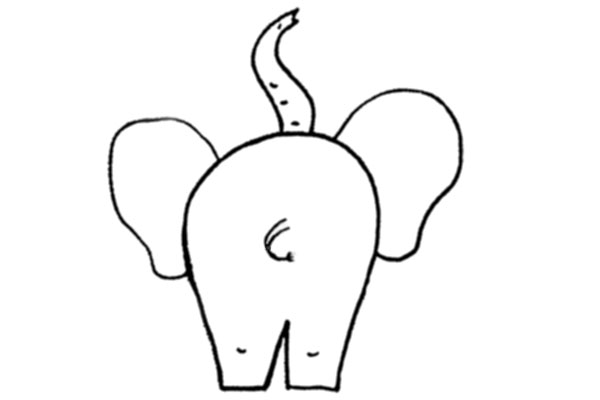
\includegraphics[scale=1.5]{images/slon.jpg}
\end{center}

\item
Укажите названия букв греческого алфавита и запишите соответствующие заглавные буквы:
\[\alpha, \zeta, \eta, \theta\].

\end{enumerate}

\subsection{Контрольная номер 1, базовый поток, 26.10.2015, решения}

\begin{enumerate}
\item
\begin{enumerate}
\item[$\alpha$)] Найдём вероятности каждого события: $\P(A) = 1/2$, $\P(B) = 1/2$, $\P(C) = 1/2$.

Проверим попарную независимость:
\begin{itemize}
\item $\P(A \cap B) = 1/4$, $\P(A) \cdot \P(B) = 1/2 \cdot 1/2 = 1/4$
\item $\P(A \cap C) = 1/4$, $\P(A) \cdot \P(C) = 1/2 \cdot 1/2 = 1/4$
\item $\P(B \cap C) = 1/4$, $\P(B) \cdot \P(C) = 1/2 \cdot 1/2 = 1/4$
\end{itemize}
Значит, события попарно независимы.
\item[$\beta$)] События $A_1, A_2, A_3$ называются независимыми в совокупности, если $\P(A_1 \cap A_2 \cap A_3) = \P(A_1) \cdot \P(A_2) \cdot \P(A_3)$.

В нашем случае: $\P(A \cap B \cap C) = 0$, $ \P(A) \cdot \P(B) \cdot \P(C) =  \frac{1}{2} \cdot \frac{1}{2} \cdot \frac{1}{2} $, следовательно, события
не являются независимыми в совокупности.
\end{enumerate}
\item
\begin{enumerate}
\item[$\alpha$)] Воспользуемся формулой полной вероятности:
\begin{multline*}
\P(\text{выпала «6»}) = \P(\text{выпала «6»} \mid \text{взят белый кубик}) \cdot \P(\text{взят белый кубик}) + \\
+ \P(\text{выпала «6»} \mid \text{взят красный кубик}) \cdot \P(\text{взят красный кубик}) = \\
= \frac{1}{6} \cdot \frac{1}{2} + \frac{1}{3} \cdot \frac{1}{2} = \frac{1}{4}
\end{multline*}
\item[$\beta$)] Воспользуемся формулой условной вероятности и результатом предыдущего пункта:
\begin{multline*}
\P(\text{взят красный кубик} \mid \text{выпала «6»}) = \frac{\P(\text{взят красный кубик} \cap \text{выпала «6»})}{\P(\text{выпала «6»})} =  \\
= \frac{\frac{1}{2}\cdot \frac{1}{3}}{\frac{1}{4}} = \frac{2}{3}
\end{multline*}
\end{enumerate}
\item
\begin{enumerate}
\item[$\alpha$)] Совместное распределение имеет вид:
\begin{center}
\begin{tabular}{@{}lllllll@{}}
\toprule
$\eta$ $\backslash$ $\xi$ & $1$                            & $2$                            & $3$                            & $4$                            & $5$                            & $6$                            \\ \midrule
$1$           & $\frac{2}{15}\cdot\frac{1}{6}$ & $\frac{2}{15}\cdot\frac{1}{6}\mbox{*}$  & $\frac{2}{15}\cdot\frac{1}{6}\mbox{*}$   & $\frac{2}{15}\cdot\frac{1}{6} \mbox{*}$   & $\frac{2}{15}\cdot\frac{1}{6} \mbox{*}$   & $\frac{1}{3}\cdot\frac{1}{6} \mbox{*}$   \\
$2$           & $\frac{2}{15}\cdot\frac{1}{6}$ & $\frac{2}{15}\cdot\frac{1}{6}$ & $\frac{2}{15}\cdot\frac{1}{6}\mbox{*}$   & $\frac{2}{15}\cdot\frac{1}{6}\mbox{*}$   & $\frac{2}{15}\cdot\frac{1}{6}\mbox{*}$   & $\frac{1}{3}\cdot\frac{1}{6} \mbox{*}$   \\
$3$           & $\frac{2}{15}\cdot\frac{1}{6}$ & $\frac{2}{15}\cdot\frac{1}{6}$ & $\frac{2}{15}\cdot\frac{1}{6}$ & $\frac{2}{15}\cdot\frac{1}{6} \mbox{*}$   & $\frac{2}{15}\cdot\frac{1}{6} \mbox{*}$   & $\frac{1}{3}\cdot\frac{1}{6} \mbox{*}$   \\
$4$           & $\frac{2}{15}\cdot\frac{1}{6}$ & $\frac{2}{15}\cdot\frac{1}{6}$ & $\frac{2}{15}\cdot\frac{1}{6}$ & $\frac{2}{15}\cdot\frac{1}{6}$ & $\frac{2}{15}\cdot\frac{1}{6} \mbox{*}$ & $\frac{1}{3}\cdot\frac{1}{6} \mbox{*}$   \\
$5$           & $\frac{2}{15}\cdot\frac{1}{6}$ & $\frac{2}{15}\cdot\frac{1}{6}$ & $\frac{2}{15}\cdot\frac{1}{6}$ & $\frac{2}{15}\cdot\frac{1}{6}$ & $\frac{2}{15}\cdot\frac{1}{6}$ & $\frac{1}{3}\cdot\frac{1}{6} \mbox{*}$   \\
$6$           & $\frac{2}{15}\cdot\frac{1}{6}$ & $\frac{2}{15}\cdot\frac{1}{6}$ & $\frac{2}{15}\cdot\frac{1}{6}$ & $\frac{2}{15}\cdot\frac{1}{6}$ & $\frac{2}{15}\cdot\frac{1}{6}$ & $\frac{1}{3}\cdot\frac{1}{6}$ \\ \bottomrule
\end{tabular}
\end{center}
\item[$\beta$)] $\P(\text{выиграет белый кубик}) = (6 + 5 + 4 + 3 + 2) \cdot \frac{2}{15}\cdot\frac{1}{6} + 1 \cdot \frac{1}{3}\cdot\frac{1}{6} = \frac{1}{2}$.

Значит, Пете безразлично, какой кубик брать.
\item[$\gamma)$] $F_{\zeta}(x) = \P(\zeta \leq x)$

Выпишем таблицу распределения случайной величины $\zeta$:

\begin{tabular}{@{}lcccccc@{}}
\toprule
$\zeta$     & $1$                              & $2$                                      & $3$                                      & $4$                                      & $5$                                      & $6$                                                                              \\ \midrule
$\P(\cdot)$ & $\frac{2}{15} \cdot \frac{1}{6}$ & $\frac{2}{15} \cdot \frac{1}{6} \cdot 3$ & $\frac{2}{15} \cdot \frac{1}{6} \cdot 5$ & $\frac{2}{15} \cdot \frac{1}{6} \cdot 7$ & $\frac{2}{15} \cdot \frac{1}{6} \cdot 9$ & $\frac{1}{3} \cdot \frac{1}{6} \cdot 6 + \frac{2}{15} \cdot \frac{1}{6} \cdot 5$ \\ \bottomrule
\end{tabular}

Тогда функция распределения имеет вид:
\[
F_{\zeta}(x) =
\begin{cases}
0 & x \leq 1 \\
\frac{1}{45} & 1 < x \leq 2 \\
\frac{4}{45} & 2 < x \leq 3 \\
\frac{9}{45} & 3 < x \leq 4 \\
\frac{16}{45} & 4 < x \leq 5 \\
\frac{25}{45} & 5 < x \leq 6 \\
1 & x > 6
\end{cases}
\]
\item[$\delta$)] $\E(\zeta) = \frac{2}{15} \cdot \frac{1}{6} \cdot 1 + \frac{2}{15} \cdot \frac{1}{6} \cdot 3 \cdot 2 + \frac{2}{15} \cdot \frac{1}{6} \cdot 5 \cdot 3 + \frac{2}{15} \cdot \frac{1}{6} \cdot 7 \cdot 4 + \frac{2}{15} \cdot \frac{1}{6} \cdot 9 \cdot 5 + \frac{1}{3} \cdot \frac{1}{6} \cdot 6 + \frac{2}{15} \cdot \frac{1}{6} \cdot 6 = \frac{43}{9} \approx 4.8 $
\end{enumerate}
\item Пусть $x$ — вероятность того, что мужчина честно любит петь в душе.

Распишем по формуле полной вероятности вероятность получить ответ «да»:
\begin{multline*}
P(\text{ответ «Да»}) = 1 \cdot \P(\text{выпала «6»}) + x \cdot(\P(\text{выпала «2»}) + \P(\text{выпала «3»}) +  \\
+ \P(\text{выпала «4»}) + \P(\text{выпала «5»})) = 1 \cdot \frac{1}{6} + x \cdot \frac{4}{6} \Rightarrow x = \frac{3}{4}
\end{multline*}
Тогда истинный процент «певцов» составляет $75 \%$
\item Предположим, что ваше имя — Студент (7 букв), а фамилия — Идеальный (9 букв).
\begin{enumerate}
\item[$\alpha$)] $\P(\text{напишет фаимлию правильно}) = (0.9)^9$
\item[$\beta$)] $\P(\text{ровно 2 ошибки в имени}) = C_{7}^2 \cdot 0.1^2 \cdot 0.9^5$
\item[$\gamma$)] Наиболее вероятное число ошибок — 1
\item[$\delta$)] $\P(\text{допустит хотя бы одну ошибку}) = 1 - \P(\text{не допустит ни одной ошибки}) = 1 - (0.9)^{16}$
\end{enumerate}
\item
\begin{enumerate}
\item[$\alpha$)] Из условия $\int_{0}^{1} (cy^2 + y) dy = 1$ получаем, что $c=3/2$.
\item[$\beta$)]
$F_{Y} (y) =
\begin{cases}
1 & y > 1 \\
\frac{y^3 + y^2}{2} & 0 < y \leq 1 \\
0 & y < 0
\end{cases} $
\item[$\gamma$)] $\P(Y < 0.5) = \int_{0}^{0.5} \left(\frac{3}{2} y^2 + y   \right) dy = \frac{3}{16}$
\item[$\delta$)] $F_{Y} (y) = 0.5 \Rightarrow y \approx 0.75 $
\item[$\epsilon$)] $\P(Y > 0.5 \mid Y \geq 0.25) = \frac{\P(Y > 0.5)}{\P(Y \geq 0.25)} = \frac{1 - \frac{3}{16}}{\int_{0.25}^{1} \left(\frac{3}{2} y^2 + y   \right) dy} = \frac{104}{123}$
\end{enumerate}
\item
\begin{enumerate}
\item[$\alpha$)] $\P(\text{кисточка окажется на слоне}) = \frac{1}{1.5} = \frac{2}{3}$
\item[$\beta$)] $f_{\xi, \eta}(x, y) = \frac{1}{1.5}$
\item[$\gamma$)] $f_{\xi} (x) = \int_{0}^{1} \frac{1}{1.5} dy = 1.5$

$f_{\eta}(y) = \int_{0}^{1.5} \frac{1}{1.5} dx = 1$
\item[$\delta$)] Да, поскольку $ f_{\xi} (x) \cdot f_{\eta}(y) = f_{\xi, \eta}(x, y)$
\item[$\epsilon$)] $f_{\xi+\eta} (t) = \int_{-\infty}^{+\infty} f_{\xi}(u) f_{\eta}(t-u) du $
\end{enumerate}
\end{enumerate}


\subsection{Праздник номер 1, исследователи, индивидуальный тур}

\begin{enumerate}
\item Для разминки вспомним греческий алфавит!

\begin{enumerate}
\item По-гречески — Σωκρατης, а по-русски — \underline{\hspace{2cm}}
\item Изобразите прописные и строчные буквы: эта \underline{\hspace{2cm}}, дзета \underline{\hspace{2cm}}, вега \underline{\hspace{2cm}}, шо \underline{\hspace{2cm}}. Если такой буквы в греческом нет, то поставьте прочерк.
\item Назовите буквы: τ \underline{\hspace{2cm}}, θ \underline{\hspace{2cm}}, ξ \underline{\hspace{2cm}}.
%\item Если пересчитать все буквы в греческом алфавите, то их окажется ровно \underline{\hspace{2cm}} %24
\end{enumerate}

\item Подбрасываются 2 симметричные монеты. Событие $A$ — на первой монете выпал герб, событие $B$ — на второй монете выпал герб, событие $C$ — монеты выпали разными сторонами.
\begin{enumerate}
\item Будут ли эти события попарно независимы?
\item Сформулируйте определение независимости в совокупности для трех событий
\item Являются ли события $A$, $B$, $C$ независимыми в совокупности?
\end{enumerate}


\item Имеются два игральных кубика: \textbf{красный} со смещенным центром тяжести, так что вероятность выпадения «6» равняется 1/3, а оставшиеся грани имеют равные шансы на появление и
правильный \textbf{белый} кубик.  Петя случайным образом выбирает кубик и подбрасывает его.
\begin{enumerate}
\item Вероятность того, что выпадет «6», равна \underline{\hspace{2cm}}
\item Вероятность того, что Петя взял красный кубик, если известно, что выпала шестерка, равна \underline{\hspace{2cm}}
\item Если бы в эксперименте Петя подбрасывал  бы кубик не один раз, а 60 раз, то безусловное математическое ожидание количества выпавших шестёрок равнялось бы \underline{\hspace{2cm}}
\end{enumerate}


\begin{comment}
\item Неразменный пятак всегда выпадает «орлом». У Александра Привалова в кармане один неразменный пятак и два обычных, равновероятно выпадающих «орлом» и «решкой». Привалов достаёт одну из монет наугад не глядя.
\begin{enumerate}
\item Вероятность того, что он достанет неразменный пятак равна \underline{\hspace{2cm}} % 1/3
\item Не глядя на монету, Привалов подкидывает её. Вероятность того, что она выпадет  «орлом», равна \underline{\hspace{2cm}} % 2/3
%\item Если бы эту случайную монету подкинуть не один раз, а 10, то математическое ожидание числа «орлов» равнялось бы \underline{\hspace{2cm}} % 20/3
\item Наконец Привалов глядит на упавшую монету и видит, что выпал «орёл». Вероятность того, что монета — неразменный пятак, равна \underline{\hspace{2cm}}
\end{enumerate}
\end{comment}

\item Винни-Пуху снится сон, будто он спустился в погреб, а там бесконечное количество горшков. Каждый из них независимо от других может оказаться либо пустым с вероятностью $0.8$, либо с мёдом с вероятностью $0.2$. Винни-Пух начинает перебирать горшки по очереди в поисках полного. Хотя у него в голове и опилки, Винни-Пух два раза в один и тот же горшок заглядывать не будет.
\begin{enumerate}
\item Вероятность того, что все горшки окажутся пустыми равна \underline{\hspace{2cm}}
\item Вероятность того, что полный горшок будет найден ровно с шестой попытки, равна \underline{\hspace{2cm}}
\item Вероятность того, что полный горшок будет найден на шестой попытке или ранее, равна \underline{\hspace{2cm}}
%\item Математическое ожидание числа перебранных горшков равняется \underline{\hspace{2cm}} % 5
\end{enumerate}

\item На самом деле у Винни-Пуха в погребе стоит 10 горшков. Каждый из них независимо от других может оказаться либо пустым с вероятностью $0.8$, либо с мёдом с вероятностью $0.2$.
\begin{enumerate}
\item Все десять горшков окажутся пустыми с вероятностью \underline{\hspace{2cm}}
\item Ровно $7$ горшков из десяти окажутся пустыми с вероятностью \underline{\hspace{2cm}}
\item Математическое ожидание числа горшков с мёдом равно \underline{\hspace{2cm}}
\end{enumerate}


\begin{comment}
\item Внутри треугольника с вершинами $(0,0)$, $(2,5)$ и $(8,0)$ случайно равномерно по площади выбирается точка. Пусть $X$ и $Y$ — абсцисса и ордината этой случаной точки.
\begin{enumerate}
\item Вероятность того, что $X>5$ равна \underline{\hspace{2cm}}.
\item Вероятность того, что $X>5$ и одновременно $Y<3$ равна \underline{\hspace{2cm}}.
\item Вероятность того, что $X>5$ если известно, что $Y<3$ равна \underline{\hspace{2cm}}.
\item События $X>5$ и $Y<3$ являются \underline{\hspace{1cm}}висимыми.
\item Функция плотности величины $X$ равна \underline{\hspace{2cm}}
\end{enumerate}
\end{comment}

\item В галактике Флатландии все объекты двумерные. На планету Тау-Слона (окружность) в случайных точках независимо друг от друга садятся три корабля. Любые два корабля могут поддерживать прямую связь между собой, если центральный угол между ними меньше прямого.

\begin{enumerate}
\item Вероятность того, что первый и второй корабли могут поддерживать прямую связь равна \underline{\hspace{2cm}}
\item Вероятность того, что все корабли смогут поддерживать прямую связь друг с другом равна \underline{\hspace{2cm}}
\item Вероятность того, что все корабли смогут поддерживать прямую связь друг с другом, если первый и второй корабль могут поддерживать прямую связь, равна \underline{\hspace{2cm}}
\end{enumerate}
Подсказка: во Флатландии хватит рисунка на плоскости, ведь координату третьего корабля можно принять за\ldots



\item Время (в часах), за которое студенты выполняют экзаменационное задание является случайной величиной $X$ с функцией плотности
\[
f(x)=\begin{cases}
3x^2, \, \text{ если } x \in [0;1] \\
0, \, \text{ иначе }
\end{cases}
\]

\begin{enumerate}
\item Функция распределения случайной величины $X$ равна \underline{\hspace{2cm}}
\item Вероятность того, что случайно выбранный студент закончит работу менее чем за полчаса равна \underline{\hspace{2cm}}.
\item Медиана распределения равна \underline{\hspace{2cm}}
\item Вероятность того, что студент, которому требуется по меньшей мере 15 минут для выполнения задания, справится с ним более, чем за 30 минут, равна \underline{\hspace{2cm}}
\item Функция распределения случайной величины $Y=1/X$ равна \underline{\hspace{2cm}}
\item Функция плотности случайной величины $Y=1/X$ равна \underline{\hspace{2cm}}
\end{enumerate}

\end{enumerate}

\subsection{Индивидуальный тур, решение}

\begin{enumerate}
\item Сократ, эта — Η, η, дзета — Ζ, ζ, вега — нет, шо — ϸ, τ — тау, θ — тета, ξ — кси.
Греческая буква шо, ϸ, была введена Александром Македонским и ныне вышла из употребления. По крайней мере, в греческом :) Заглавная примерно такая же, только её utf-код 03f7 не поддерживается шрифтом Linux Libertine.


\item да; события независимы в совокупности, если для любого поднабора событий $A_1$, \ldots, $A_k$ выполняется равенство $\P(A_1 \cap A_2 \cap \ldots \cap A_k) = \P(A_1) \cdot \ldots \cdot \P(A_k)$; нет
\item $1/4$, $2/3$, $15$
\item $0$, $0.8^5\cdot 0.2$, $1-0.8^6$
\item $0.8^{10}$, $C_{10}^3 0.2^3 0.8^7$, $2$
\item $1/2$, $3/16$, $3/8$
\begin{enumerate}
\item
\begin{flalign*}
F_X(x) &= \begin{cases}
0, \, x<0 \\
x^3, \, x \in [0;1] \\
1, \, x>1
\end{cases}&&
\end{flalign*}
\item $1/8$
\item $2^{-1/3}$
\item $56/63$
\item
\begin{flalign*}
F_Y(y) &= \begin{cases}
0, \, y<0 \\
1-1/y^3, \, y>0
\end{cases}&&
\end{flalign*}
\item
\begin{flalign*}
f_Y(y) &= \begin{cases}
0, \, y<0 \\
3y^{-4}, \, y>0
\end{cases}&&
\end{flalign*}

\end{enumerate}

\end{enumerate}

\subsection{Регата, исследователи, командный тур}

\begin{enumerate}
\item Восьминогий Кракен. У Кракена 8 ног-шупалец. Если отрубить одно щупальце, то в замен него с вероятностью $1/4$ вырастает новое; с вероятностью $1/4$ вырастает два новых; с вероятностью $1/2$, слава Океану, не вырастает ничего.

Против Кракена бьётся сам Капитан! Он наносит точные удары и безупречно умело уворачивается от ударов Кракена.

\begin{enumerate}
\item Какова вероятность того, что Капитан победит, отрубив ровно 10 щупалец?
\item Какова вероятность того, что бой Кракена и Капитана продлится вечно?
\item Сколько щупалец в среднем отрубит Капитан прежде чем победит?
\end{enumerate}

\item Разбавленный ром. Пират Злопамятный Джо очень любит неразбавленный ром. Из-за
того, что он много пьёт, у него проблемы с памятью, и он помнит не
больше, чем три последних пинты. Хозяин таверны с вероятностью 1/4 разбавляет
каждую подаваемую пинту рома. Если по ощущением Джо половина выпитых
пинт или больше была разбавлена, то он разносит таверну к чертям
собачьим.


\begin{enumerate}
\item Какова вероятность того, что хозяин таверны не успеет подать Джо третью пинту рома?
\item Сколько в среднем пинт выпьет Джо, прежде чем разнесёт таверну?
\end{enumerate}

\item $XY$ в степени $Z$. Чтобы поступить на службу Её Величества, пиратам предлагается следующая задача. Случайные величины $X$, $Y$ и $Z$ равномерны на отрезке $[0;1]$ и независимы.

\begin{enumerate}
\item Найдите функцию распределения случайной величины $-\ln X$
\item Найдите функцию распределения случайной величины $-(\ln X + \ln Y)$
\item Найдите функцию распределения случайной величины $-Z(\ln X + \ln Y)$
\item Какое распределение имеет случайная величина $(XY)^Z$?
\end{enumerate}

\item Тортики. Пираты очень любят тортики и праздновать день рождения! Если хотя бы у одного пирата на корабле день рождения, то все, включая капитана, празднуют и кушают тортики. Корабль в праздничный день дрейфует под действием ветра и не факт, что в нужном направлении.

\begin{enumerate}
\item Сколько пиратов нужно нанять капитану, чтобы ожидаемое количество праздничных дней было равно 100?
\item Сколько пиратов нужно нанять капитану, чтобы максимизировать ожидаемое количество рабочих пирато-дней (произведение числа пиратов на число рабочих дней)?
\end{enumerate}


\item Девятый вал. На побережье пиратского острова одна за одной набегают волны. Высота каждой волны — равномерная на $[0;1]$ случайная величина. Высоты волн независимы. Пираты называют волну «большой», если она больше предыдущей и больше следующей. Пираты называют волну «рекордной», если она больше всех предыдущих волн от начала наблюдения. Обозначим события $B_i= \{ i\text{-ая волна была большой} \}$ и $R_i=\{ i\text{-ая волна была рекордной} \}$.

\begin{enumerate}
\item Найдите $\P(R_{100})$, $\P(B_{100})$
\item Капитан насчитал 100 волн. Сколько в среднем из них были «рекордными»?
\item Найдите $\P(R_{99} | R_{100})$, $\P(R_{100}|B_{100})$
\end{enumerate}


\item Три сундука. Три пирата, Генри Рубинов, Френсис Пиастров и Эдвард Золотов играют одной командой в игру. В комнате в ряд, слева направо, стоят в случайном порядке три закрытых внешне неотличимых сундука: с рубинами, пиастрами и золотом. Общаться после начала игры они не могут, но могут заранее договориться о стратегии. Они заходят в комнату по очереди. Каждый из них может открыть два сундука по своему выбору. После каждого пирата комната возвращается уборщицей идеально точно в исходное состояние. Если Рубинов откроет коробку с рубинами, Писатров — с пиастрами, а Золотов — с золотом, то их команда выигрывает. Если хотя бы один из пиратов не найдёт свою цель, то их команда проигрывает.

\begin{enumerate}
\item Какова вероятность выигрыша, если все пираты пробуют открыть первый и второй сундуки?
\item Какова оптимальная стратегия?
\item Какова вероятность выигрыша при использовании оптимальной стратегии?
\end{enumerate}






\end{enumerate}

\subsection{Регата, исследователи, командный тур, решение}

\begin{enumerate}

\item Если отрублено 10 щупалец, значит либо был один удар породивший два новых щупальца, либо было два удара, породивших по одному новому, а все остальные удары не порождали новых щупалец.

Искомая вероятность равна: $8\cdot 0.5^9 \cdot 0.25^1 + C_8^2 0.5^8 0.25^2$.

Вероятность вечного боя равна нулю. Достаточно доказать, что с вероятностью один за конечное время побеждается одноногий Кракен. А эта вероятность удовлетворяет уравнению: $p=\frac{1}{4}p + \frac{1}{4}p^2 + \frac{1}{2} 1$. Единственный осмысленный корень у этого уравнения — $1$.

Замечаем, что на победу над $k$-шупальцевым Кракеном уходим в $k$ раз больше ударов в среднем чем на победу на $1$-щупальцевым. Отсюда:

\[
e_1=1 + 0.5\cdot 0 + 0.25\cdot e_1 + 0.25 \cdot 2e_1
\]

Решаем, получаем $e_1=4$ и $e_8=32$

\item Либо первая пинта разбавлена, либо первая неразбавлена, а вторая разбавлена, то есть
\[
0.25 + 0.75\cdot 0.25 =0.4375
\]

Рисуем граф:


Составляем систему (индекс — количество выпитых неразбавленных пинт):

\[
\begin{cases}
e_0=\frac{1}{4} + \frac{3}{16}2 + \frac{9}{16}(2+e_2) \\
e_2=1+\frac{3}{4}e_2 + \frac{1}{4}e_0
\end{cases}
\]

Находим $e_0=64/7\approx 9$

\item Начало из домашки! Для $t>0$:
\[
\P(-\ln X \leq t)=\P(\ln X > -t)=\P(X > e^{-t})=1-e^{-t}
\]

Итого,
\[
F_{-\ln X}(t)=\begin{cases}
0, \, t < 0 \\
1-e^{-t}, \, t \geq 0
\end{cases}
\]

Из геометрических соображений легко найти $\P(XY < a)$ для $a\in (0;1)$:
\[
\P(XY < a)=a + \int_a^1 \frac{a}{x} \, dx=a-a\ln a
\]

Переходим ко второму пункту, для $t>0$:
\[
\P(-(\ln X + \ln Y) < t)=\P(XY > e^{-t})= 1-e^{-t} -t e^{-t}
\]

Итого:
\[
F_{-\ln X - \ln Y}(t)=\begin{cases}
0, \, t < 0 \\
1-e^{-t} - te^{-t}, \, t \geq 0
\end{cases}
\]

После дифференциирования получаем функцию плотности для $S=-\ln X - \ln Y$:

\[
f_S(s)=\begin{cases}
0, \, s < 0 \\
se^{-s}, \, s \geq 0
\end{cases}
\]

Приближаемся к финальной вероятности:

\[
\P(ZS > t)= \int_t^{\infty} \int_{t/s}^1  se^{-s} \, dz\, ds=
\int_t^{\infty} (s-t)\cdot e^{-s} \, ds= \ldots = e^{-t}
\]

Сравниваем результат с первым пунктом и приходим к выводу, что величина $(XY)^Z$ имеет равномерное распределение на $[0;1]$.

\item Если нанято $n$ пиратов, то вероятность, того, что в конкретный день все работают равна $(364/365)^n$. Следовательно, ожидаемое количество праздничных дней равно $365(1-(364/365)^n)$.

Решаем уравнение

\[
1-(364/365)^n=100/365
\]

Получаем,
\[
n=\frac{\ln 265- \ln 365}{ \ln 364 - \ln 365}\approx 117
\]

Ожидаемое количество рабочих пирато-дней равно: $365n(364/365)^n$.

Получаем
\[
n^*=1/(\ln 365 - \ln 364)\approx 364
\]

\item
\begin{enumerate}
\item $\P(R_{100})=1/100$ (максимум из 100 величин должен плюхнуться на сотое место), $\P(B_{100})=1/3$ (максимум из трёх величин должен плюхнуться на второе место)
\item $\E(X)=1+\frac{1}{2} + \frac{1}{3}+\ldots + \frac{1}{100}\approx \ln 100 \approx 4.6$. Т.к. $X=X_1+X_2+\ldots + X_{100}$ и $\E(X_i)=1/i$.
\item $\P(R_{99} | R_{100})=1/99$, $\P(R_{100}|B_{100})=3/101$

Для проверки: $\P(R_{99} \cap R_{100})=98!/100!$ ($100!$ — всего перестановок, $98!$ — первые 98 можно переставлять свободно, а в конце должны идти второй наибольшое и наибольшее). $\P(R_{100} \cap B_{100})=1/101$ (максимум из 101 числа плюхнется на 100ое место).
\end{enumerate}

\item Если все пираты открывают первый и второй сундуки, то вероятность выигрыша равна нулю.

Оптимальная стратегия (одна из). Три пирата заранее договариваются, о названиях сундуков. Они называют эти три сундука (ещё до игры)  «рубиновым», «пиастровым» и «золотым». Генри Рубинов должен начать с открытия рубинового сундука, Френсис Пиастров — с пиастрового, Эдвард Золотов — с золотого. Далее каждый пират должен открыть тот сундук, на который указывает предмет, лежащий в первом открытом им сундуке. Например, если Генри Рубинов, открыв сначала рубиновый сундук обнаруживает там пиастры, он должен открывать пиастровый сундук.

Вероятность победы при такой стратегии легко находится перебором 6 возможных вариантов и равна\ldots Та-дам!!! $2/3$.




\end{enumerate}


\subsection{Контрольная номер 2, поток Арктура, 12.12.2015}

Продолжительность: 1 час 20 минут

\begin{enumerate}
\item Функция плотности случайного вектора $\xi=(\xi_1, \xi_2)^T$ имеет вид
\[
f(x,y)=\begin{cases}
0.5x + 1.5y, \text{ если } 0<x<1, \; 0<y<1 \\
0, \text{ иначе }
\end{cases}
\]
Найдите:
\begin{enumerate}
\item Математическое ожидание $\E(\xi_1 \cdot \xi_2)$
\item Условную плотность распределения $f_{\xi_1|\xi_2} (x|y)$
\item Условное математическое ожидание $\E(\xi_1| \xi_2=y)$
\item Константу $k$, такую, что функция $h(x,y)=kx\cdot f(x,y)$ будет являться совместной функцией плотности некоторой пары случайных величин
\end{enumerate}

\item На курсе учится очень много студентов. Вероятность того, что случайно выбранный студент по результатам рубежного контроля имеет хотя бы один незачет равна $0.2$. Пусть $\xi$ и $\eta$ — число студентов с незачетами и без незачетов в случайной группе из $10$ студентов. Найдите $\Cov(\xi,\eta)$, $\Corr(\xi,\eta)$, $\Cov(\xi-\eta,\xi)$. Являются ли случайные величины $\xi-\eta$ и $\xi$ независимыми?

\item Доходности акций компаний А и В – случайные величины $\xi$ и $\eta$. Известно, что $\E(\xi)=1$, $E(\eta)=1$, $\Var(\xi)=4$, $\Var(\eta)=9$, $\Corr(\xi,\eta)=-0.5$. Петя принимает решение потратить свой рубль на акции компании А, Вася — 50 копеек на акции компании А и 50 копеек на акции компании В, а Маша  принимает решение вложить свой рубль в портфель $R=\alpha\xi+(1-\alpha)\eta$, $(0 \leq \alpha \leq 1)$, обладающий минимальным риском. Найдите $\alpha$, ожидаемые доходности и риски портфелей Пети, Васи и Маши.

\item Будем считать, что рождение мальчика и девочки равновероятны.
\begin{enumerate}
\item Оцените с помощью неравенства Маркова вероятность того, что среди тысячи новорожденных младенцев, мальчиков будет более 75\%.
\item Оцените с помощью неравенства Чебышёва вероятность того, что доля мальчиков среди тысячи новорожденных младенцев будет отличаться от 0.5 более, чем на 0.25
\item С помощью теоремы Муавра-Лапласа вычислите вероятность из предыдущего пункта.
\end{enumerate}

\item Сейчас валютный курс племени «Мумба» составляет 100 оболов за один рубль. Изменение курса за один день — случайная величина $\delta_i$ с законом распределения:

\begin{center}
\begin{tabular}{lrrr}
\toprule
$\delta_i$ & $-1$ & $0$ & $2$ \\ \midrule
$\P(\cdot)$ & $0.25$ & $0.5$ & $0.25$ \\
\bottomrule
\end{tabular}
\end{center}

Найдите вероятность того, что через полгода (171 день) рубль будет стоить более 250 оболов, если ежедневные изменения курса происходят независимо друг от друга.

\item \textbf{Бонусная задача}

Число посетителей, зашедших в магазин в течении дня — пуассоновская случайная величина с параметром $\lambda$. Каждый из посетителей совершает покупку с вероятностью $p$, не зависимо от других посетителей. Найдите математическое ожидание числа человек, совершивших покупку.

\end{enumerate}


\subsection{Контрольная номер 2, поток Арктура, 12.12.2015, решение}

\begin{enumerate}
\item
\begin{enumerate}
\item $ \E({\xi_1 \cdot \xi_2}) = \int_{0}^1 \int_0^1 xy f(x,y) \, dx \, dy = \int_0^1 \int_0^1 \frac{1}{2}\cdot x^2y + \frac{3}{2}\cdot xy^2 \, dx \, dy = \int_{0}^1 \frac{y}{6} + \frac{3y^2}{4} \,dy = \frac{1}{3}$
\item $f_{\xi_1 | \xi_2} (x | y) = \frac{f_{\xi_1, \xi_2}(x, y)}{f_{\xi_2}(y)} = \frac{0.5x + 1.5y}{0.25 + 1.5y}, \text{ при } y \in (0,1)$
\item
\begin{multline*}
\E(\xi_1 | \xi_2 = y) = \int_0^1 x f_{\xi_1 | \xi_2} (x | y) dx = \\
= \int\limits_{0}^{1}  x \frac{0,5x + 1,5y}{0,25 + 1,5y} dx = \frac{1}{0,25 + 1,5y}  \left. \left( \dfrac{0,5x^3}{3} +  \dfrac{1,5yx^2}{2} \right) \right|_0^1  =  \frac{1/6 + 3/4y}{0,25 + 1,5y}
\end{multline*}
\item
Для того, чтобы функция являлась совместной плотностью для пары случайных величин, должно выполнятся следующее:
\[
\int_{\Omega} kx f(x,y) \, dx \, dy = 1
\]
Вычислим, чему равняется левая часть:
\[
1 = \int_{\Omega} kx f(x,y) \, dx \, dy = \int_{0}^1 \int_{0}^1 kx \left(\frac{x + 3y}{2}\right) dx \, dy = \int_{0}^1 \frac{k}{6} + \frac{3ky}{4} \, dy = \frac{k}{6} + \frac{3k}{8} \Rightarrow
\]
\[
k = \frac{24}{13}
\]
\end{enumerate}
\item Заметим, что $\xi + \eta = 10$, тогда $\Cov(\xi, \eta) = \Cov(\xi, 10-\xi) = -\Var(\xi)$.

Представим случайную величину $\xi$ в виде суммы случайных величин $\xi = \xi_1 + \ldots + \xi_{10}$, где
\[
\xi_i = \begin{cases}
1, & \text{если у студента есть хотя бы один незачёт}, p=0.2 \\
0, & \text{иначе}, p=0.8
\end{cases} \quad i = 1, \ldots, 10
\]

Поскольку результаты каждого из стуентов независимы, $\Var(\xi) = 10\Var(\xi_1)$
\[
\Cov(\xi, \eta) = -10(1^2 \cdot 0.2 - (1\cdot 0.2)^2) = -1.6
\]

Так как случайные величины $\xi$ и $\eta$ связаны соотношением $\xi = 10 - \eta$, $\Corr(\xi, \eta)=-1$.

Подставив в $\Cov(\xi - \eta, \xi)$ выражение $\eta = 10 - \xi$, получим:
\[
\Cov(\xi - \eta, \xi) = 2 \Cov(\xi, \xi) = 2 \cdot 0.16 = 0.32
\]
Случайные величины $\xi - \eta$ и $\xi$ не являются независиыми.
\item Найдем ожидаемую доходность и риск портфеля $R = \alpha \xi + (1-\alpha) \eta$ для любого $\alpha$, тогда при $\alpha = 1$ получим результаты Пети, при $\alpha = 0.5$ — результаты Васи.
\[
\E R = \alpha + (1-\alpha) = 1 \: \, \forall \, \: \alpha \in [0,1]
\]

Находим дисперсию:
\[
\Var(R) = \alpha^2 \cdot 4 + (1-\alpha)^2 \cdot 9 - 6\alpha (1-\alpha) = 19\alpha^2 -24\alpha + 9 \to \min_{\alpha} \Rightarrow
\]

Теперь, найдем оптимальное $\alpha$:
\[
\alpha = \frac{24}{38}
\]

Финальные цифры:
\[
\begin{cases}
\Var(R)^{P} = 4 \Rightarrow \sigma_{P} = 2 \\
\Var(R)^{V} = 1.75 \Rightarrow \sigma_{V} \approx 1.32 \\
\Var(R)^{M} = \frac{27}{19} \Rightarrow \sigma_{M} \approx 1.19 \\
\end{cases}
\]
\item
\begin{enumerate}
\item Пусть $S$ количество мальчиков, тогда используя \href{https://en.wikipedia.org/wiki/Markov%27s_inequality}{неравенство Маркова} получаем:
\[
\P(S \ge 750) \le \frac{\E(S)}{750} = \frac{2}{3}
\]
\item Пусть, теперь, $\overline{X}$ доля мальчиков, то есть, $\overline{X} = \sum_{i=1}^n X_i /n$, где
\[
X_i =
\begin{cases}
1, \text{ если }i\text{-ый ребёнок — мальчик }\\
0, \text{ иначе }
\end{cases}
\]
тогда используя \href{https://en.wikipedia.org/wiki/Markov%27s_inequality}{неравенство Чебышева} получаем:
\[
\P(|\overline{X} - 0.5| \ge 0.25) \le \frac{\Var(\overline{X})}{0.25^2} = \frac{1/4000}{0.25^2} = 0.004
\]
\item Вероятность из предыдущего пункта можно записать в таком виде:
\begin{multline*}
\P(|\overline{X} - 0.5| \ge 0.25) = \P(\overline{X} \ge 0.75) + \P(\overline{X} \le 0.25) = 2\P(\overline{X} \ge 0.75)=\\
= 2\P(\cN(0;1)\geq 0.25\sqrt{4000})=2\P(\cN(0;1)\geq 15.8) = 1.3 \cdot 10^{-56} \approx 0
\end{multline*}
\end{enumerate}
\item Пусть случайная величина $S$ —  это валютный курс через полгода. Заметим, что $S = 100 + \delta_1 + \ldots + \delta_{171}$.
Тогда по ЦПТ $S \sim \cN(142.75, 203.0625)$. Теперь можно искать нужную вероятность:
\[
\P(S > 250) = \P \left(\frac{S -  142.75}{\sqrt{203.0625}} > \frac{250-142.75}{\sqrt{203.0625}} \right) = \P(\cN(0, 1) > 7.6) \approx 0
\]
%\item $\lambda p$
\end{enumerate}




\subsection{Контрольная номер 2, поток Риччи, 12.12.2015}

Продолжительность: 1 час 20 минут


\begin{enumerate}
\item Функция плотности случайного вектора $\xi=(\xi_1, \xi_2)^T$ имеет вид
\[
f(x,y)=\begin{cases}
0.5x + 1.5y, \text{ если } 0<x<1, \; 0<y<1 \\
0, \text{ иначе }
\end{cases}
\]
Найдите:
\begin{enumerate}
\item Математическое ожидание $\E(\xi_1 \cdot \xi_2)$
\item Условную плотность распределения $f_{\xi_1|\xi_2} (x|y)$
\item Условное математическое ожидание $\E(\xi_1| \xi_2=y)$
\item Константу $k$, такую, что функция $h(x,y)=kx\cdot f(x,y)$ будет являться совместной функцией плотности некоторой пары случайных величин
\end{enumerate}

\item На курсе учится очень много студентов. Вероятность того, что случайно выбранный студент получит «отлично» за контрольную равна $0.2$, «хорошо» — $0.3$. Вероятности остальных результатов неизвестны. Пусть $\xi$ и $\eta$ — число отличников и хорошистов в случайной группе из $10$ студентов. Найдите $\Cov(\xi,\eta)$, $\Corr(\xi,\eta)$, $\Cov(\xi-\eta,\xi)$. Являются ли случайные величины $\xi-\eta$ и $\xi$ независимыми?

\item Доходности акций компаний А и В — случайные величины $\xi$ и $\eta$. Известно, что $\E(\xi)=1$, $E(\eta)=1$, $\Var(\xi)=4$, $\Var(\eta)=9$, $\Corr(\xi,\eta)=-0.5$. Петя принимает решение потратить свой рубль на акции компании А, Вася — 50 копеек на акции компании А и 50 копеек на акции компании В, а Маша  принимает решение вложить свой рубль в портфель $R=\alpha\xi+(1-\alpha)\eta$, $(0 \leq \alpha \leq 1)$, обладающий минимальным риском. Найдите $\alpha$, ожидаемые доходности и риски портфелей Пети, Васи и Маши.

\item Будем считать, что рождение мальчика и девочки равновероятны.
\begin{enumerate}
\item С помощью закона больших чисел определите в каком городе, большом или маленьком, больше случается таких дней, когда рождается более 75\% мальчиков.
\item Оцените с помощью неравенства Маркова вероятность того, что среди тысячи новорожденных младенцев мальчиков будет более 75\%.
\item Оцените с помощью неравенства Чебышёва вероятность того, что доля мальчиков среди тысячи новорожденных младенцев будет отличаться от 0.5 более, чем на 0.25
\item С помощью теоремы Муавра-Лапласа вычислите вероятность из предыдущего пункта.
\end{enumerate}

\item Сейчас валютный курс племени «Мумба» составляет 100 оболов за один рубль. Процентное изменение курса за один день — случайная величина $\delta_i$ с законом распределения:

\begin{center}
\begin{tabular}{lrr}
\toprule
$\delta_i$ & $-1\%$  & $1\%$ \\
$\P(\cdot)$ & $0.25$  & $0.75$ \\
\bottomrule
\end{tabular}
\end{center}

Найдите вероятность того, что через полгода (171 день) рубль будет стоить более 271 обола, если ежедневные изменения курса происходят независимо друг от друга.

\item Величины $X_1$, $X_2$, \ldots независимы и равновероятно принимают значения $-1$ и $3$.
\begin{enumerate}
\item Найдите $\plim_{n\to\infty} \frac{\sum_{i=1}^n(X_i-\bar X)^2}{n}$
\item С помощью дельта-метода найдите примерный закон распределения $\frac{\sum_{i=1}^{100}(X_i-\bar X)^2}{100}$
\end{enumerate}

\end{enumerate}

\subsection{Контрольная номер 2, поток Риччи, 12.12.2015, решение}

Решение: Аршак Минасян


\begin{enumerate}

\item
\begin{enumerate}
\item $ \E({\xi_1 \cdot \xi_2}) = \int_{0}^1 \int_0^1 xy f(x,y) \, dx \, dy = \int_0^1 \int_0^1 \frac{1}{2}\cdot x^2y + \frac{3}{2}\cdot xy^2 \, dx \, dy = \int_{0}^1 \frac{y}{6} + \frac{3y^2}{4} \,dy = \frac{1}{3}$
\item $f_{\xi_1 | \xi_2} (x | y) = \frac{f_{\xi_1, \xi_2}(x, y)}{f_{\xi_2}(y)} = \frac{0.5x + 1.5y}{0.25 + 1.5y}, \text{ при } y \in (0,1)$
\item
\begin{multline*}
\E(\xi_1 | \xi_2 = y) = \int_0^1 x f_{\xi_1 | \xi_2} (x | y) dx = \\
= \int\limits_{0}^{1}  x \frac{0,5x + 1,5y}{0,25 + 1,5y} dx = \frac{1}{0,25 + 1,5y}  \left. \left( \dfrac{0,5x^3}{3} +  \dfrac{1,5yx^2}{2} \right) \right|_0^1  =  \frac{1/6 + 3/4y}{0,25 + 1,5y}
\end{multline*}
\item
Для того, чтобы функция являлась совместной плотностью для пары случайных величин, должно выполнятся следующее:
\[
\int_{\Omega} kx f(x,y) \, dx \, dy = 1
\]
Вычислим, чему равняется левая часть:
\[
1 = \int_{\Omega} kx f(x,y) \, dx \, dy = \int_{0}^1 \int_{0}^1 kx \left(\frac{x + 3y}{2}\right) dx \, dy = \int_{0}^1 \frac{k}{6} + \frac{3ky}{4} \, dy = \frac{k}{6} + \frac{3k}{8} \Rightarrow
\]
\[
k = \frac{24}{13}
\]
\end{enumerate}
\item При расчёте ковариации применим разложение случайной величины в сумму простых случайных величин!

$\Cov(\xi, \eta) = \Cov(\xi_1 + \ldots + \xi_{10}, \eta_1 + \ldots + \eta_{10})=10\Cov(\xi_1, \eta_1)=10(0-0.2\cdot 0.3)=-0.6$

$\Var(\xi)=10\cdot 0.2\cdot 0.8=1.6 $

$\Var(\eta)=10\cdot 0.3\cdot 0.7=2.1 $

$\Corr(\xi,\eta)=-0.6/\sqrt{1.6\cdot 2.1} \approx -0.33 $

$\Cov(\xi - \eta, \xi) = \Var(\xi) - \Cov(\xi, \eta) \neq 0$

Следовательно, $\xi$ и $\eta$ зависимы.

\item Найдем ожидаемую доходность и риск портфеля $R = \alpha \xi + (1-\alpha) \eta$ для любого $\alpha$, тогда при $\alpha = 1$ получим результаты Пети, при $\alpha = 0.5$ — результаты Васи.
\[
\E R = \alpha + (1-\alpha) = 1 \: \, \forall \, \: \alpha \in [0,1]
\]

Находим дисперсию:
\[
\Var(R) = \alpha^2 \cdot 4 + (1-\alpha)^2 \cdot 9 - 6\alpha (1-\alpha) = 19\alpha^2 -24\alpha + 9 \to \min_{\alpha} \Rightarrow
\]

Теперь, найдем оптимальное $\alpha$:
\[
\alpha = \frac{24}{38}
\]

Финальные цифры:
\[
\begin{cases}
\Var(R)^{P} = 4 \Rightarrow \sigma_{P} = 2 \\
\Var(R)^{V} = 1.75 \Rightarrow \sigma_{V} \approx 1.32 \\
\Var(R)^{M} = \frac{27}{19} \Rightarrow \sigma_{M} \approx 1.19 \\
\end{cases}
\]

\item
\begin{enumerate}
\item По ЗБЧ имеем:
\[
\frac{\xi_1 + \dots + \xi_n}{n} \to \E(\xi_1) = \frac{1}{2},
\]
Поэтому, чем больше $n$ (количество жителей в городе), тем меньше таких дней, когда количество мальчиков больше $75\%.$ \\
\item Пусть $S$ количество мальчиков, тогда используя \href{https://en.wikipedia.org/wiki/Markov%27s_inequality}{неравенство Маркова} получаем:
\[
\P(S \ge 750) \le \frac{\E(S)}{750} = \frac{2}{3}
\]
\item Пусть, теперь, $\bar X$ доля мальчиков, то есть, $\overline{X} = \sum_{i=1}^n X_i /n$, где
\[
X_i =
\begin{cases}
1, \text{ если }i\text{-ый ребёнок — мальчик }\\
0, \text{ иначе }
\end{cases}
\]
тогда используя \href{https://en.wikipedia.org/wiki/Markov%27s_inequality}{неравенство Чебышева} получаем:
\[
\P(|\overline{X} - 0.5| \ge 0.25) \le \frac{\Var(\overline{X})}{0.25^2} = \frac{1/4000}{0.25^2} = 0.004
\]
\item Вероятность из предыдущего пункта можно записать в таком виде:
\begin{multline*}
\P(|\overline{X} - 0.5| \ge 0.25) = \P(\overline{X} \ge 0.75) + \P(\overline{X} \le 0.25) = 2\P(\overline{X} \ge 0.75)=\\
= 2\P(\cN(0;1)\geq 0.25\sqrt{4000})=2\P(\cN(0;1)\geq 15.8) = 1.3 \cdot 10^{-56} \approx 0
\end{multline*}
\end{enumerate}

\item

Ищем вероятность

\[
100\cdot X_1 \cdot \ldots \cdot X_{171} \geq 271
\]

Здесь $X_i$ принимают значения $0.99$ или $1.01$ с вероятностями $0.25$ и $0.75$

Берем логарифм:

\[
\sum \log X_i \geq 1
\]

Исходим из худшего случая, когда на калькуляторе нет логарифма, тогда неплохо знать, что $\log (1+\alpha) \sim \alpha$, поэтому можно считать, что $\log X_i$ принимает значения $-0.01$ и $0.01$.

Значит $\E(\log X_i)=1/200$, $\Var(\log X_i)=1/100 - 1/200^2 \approx 1/100$.

Поэтому сумма $S \sim \cN(171/200, 171/100)$ и

\[
\P(S \geq 1)=\P(\cN(0, 1) \geq 0.11) \approx 0.46
\]

\item
\begin{enumerate}
\item Используем ЗБЧ:
\[
\plim_{n \to \infty} \frac{\sum_{i=1}^n (X_i - \bar{X})^2}{n} = \plim \frac{\sum X_i^2}{n} - \plim \bar X \cdot \bar X = \E(X_1^2) - (\E(X_1))^2 = \Var(X_1) = 4
\]
\item Обозначим, $Y_i=X_i^2$, тогда наше выражение можно записать в виде:
\[
Q=\overline{Y} - (\overline{X})^2
\]

Причём, $\plim \bar Y = 5$, $\plim \bar X = 1$.

Согласно дельта-методу заменяем его на линейную аппроксимацию в окрестности предела:
\[
Q\approx 4 + (\bar Y - 5) + 2 (\bar X - 1)
\]

Стало быть, при больших $n$:

\[
\E(Q) \approx 4
\]

\begin{multline*}
\Var(Q) \approx \Var(\bar Y) + 4\Var(\bar X) + 4\Cov(\bar Y, \bar X) =\\
= \frac{1}{n} \left(\Var(Y_1) + 4 \Var(X_1) + 4\Cov(X_1, Y_1) \right) = \\
= 0.01 \cdot (16 + 4 \cdot 4 + 4 \cdot 8)= 0.64
\end{multline*}

Итого, $Q \approx \cN(4; 0.64)$

\end{enumerate}

\end{enumerate}



\subsection{Midterm, 21.12.2015}


\element{probability1}{
  \begin{questionmult}{1} %2015ready
Крошка Джон  попадает в яблочко с вероятностью $0.8$. Его выстрелы независимы. Вероятность, что он попадёт хотя бы один раз из двух равна
\begin{multicols}{3}
   \begin{choices}
      \correctchoice{$0.96$}
      \wrongchoice{$0.8$}
      \wrongchoice{$0.64$}
      \wrongchoice{$0.36$}
      \wrongchoice{$0.9$}

       \end{choices}
  \end{multicols}
  \end{questionmult}
}

\element{probability1}{
  \begin{questionmult}{2} %2015ready
Крошка Джон попадает в яблочко с вероятностью $0.8$. Его выстрелы независимы. Вероятность, что он попал оба раза, если известно, что он попал хотя бы один раз из двух, равна
   \begin{multicols}{3}
   \begin{choices}
      \correctchoice{$2/3$}
      \wrongchoice{$1/3$}
      \wrongchoice{$1/2$}
      \wrongchoice{$3/4$}
      \wrongchoice{$1/4$}

       \end{choices}
  \end{multicols}
  \end{questionmult}
}

\element{probability1}{
  \begin{questionmult}{3} %2015ready
Имеется три монетки. Две «правильных» и одна — с «орлами» по обеим сторонам. Вася выбирает одну монетку наугад и подкидывает её два раза. Вероятность того, что оба раза выпадет орел равна
    \begin{multicols}{3}
   \begin{choices}
      \correctchoice{$1/2$}
      \wrongchoice{$2/3$}
      \wrongchoice{$1/3$}
      \wrongchoice{$1/4$}
      \wrongchoice{$3/4$}

       \end{choices}
  \end{multicols}
  \end{questionmult}
}

%
% \element{probability1}{
%   \begin{questionmult}{3} %2015ready
% Крошка Джон попадает в яблочко с вероятностью $0.8$. Его выстрелы независимы. Вероятность, что он попал во второй раз, если известно, что он попал хотя бы один раз из двух, равна
%   \begin{multicols}{3}
%    \begin{choices}
%       \correctchoice{$5/6$}
%       \wrongchoice{$3/4$}
%       \wrongchoice{$2/3$}
%       \wrongchoice{$1/2$}
%       \wrongchoice{$4/5$}
%
%        \end{choices}
%   \end{multicols}
%   \end{questionmult}
% }

\element{probability1}{
  \begin{questionmult}{4} %2015ready
    Если события $A$, $B$, $C$ попарно независимы, то
    \begin{choices}
      \wrongchoice{Событие $A\cup B\cup C$ обязательно произойдёт}
      \wrongchoice{События $A$, $B$, $C$ независимы в совокупности}
      \wrongchoice{События $A$, $B$, $C$ зависимы в совокупности}
      \wrongchoice{События $A$, $B$, $C$ несовместны}
      \wrongchoice{$\P(A\cap B\cap C)=\P(A)\P(B)\P(C)$}

    \end{choices}
  \end{questionmult}
}


\element{probability1}{
  \begin{questionmult}{5} %2015ready
Случайная величина $X$ равномерна на отрезке $[0;10]$. Вероятность $\P(X>3|X<7)$ равна
    \begin{multicols}{3}
   \begin{choices}
      \correctchoice{$4/7$}
      \wrongchoice{$3/10$}
      \wrongchoice{$7/10$}
      \wrongchoice{$3/7$}
      \wrongchoice{$0.21$}

       \end{choices}
  \end{multicols}
  \end{questionmult}
}


\element{probability}{
  \begin{questionmult}{6} %2015ready
Имеется три монетки. Две «правильных» и одна — с «орлами» по обеим сторонам. Вася выбирает одну монетку наугад и подкидывает её два раза. События $A = \{ \text{Орёл выпал при первом подбрасывании} \}$ и $B =\{\text{Орёл выпал при втором подбрасывании}\}$
  \begin{multicols}{2}
   \begin{choices}
      \correctchoice{удовлетворяют соотношению $\P(A|B)\geq \P(A)$}
      \wrongchoice{независимы}
      \wrongchoice{несовместны}
      \wrongchoice{образуют полную группу событий}
       \wrongchoice{удовлетворяют соотношению $\P(A\cap B)=\P(A)+\P(B) + \P(A\cup B)$}

       \end{choices}
  \end{multicols}
  \end{questionmult}
}


\element{probability}{
  \begin{questionmult}{7} %2015ready
В квадрат вписан круг. Наудачу в квадрат бросают восемь точек. Пусть $X$ — число точек, попавших в круг. Математическое ожидание величины $X$ равно
    \begin{multicols}{3}
   \begin{choices}
      \correctchoice{$2\pi$}
      \wrongchoice{$\pi$}
      \wrongchoice{$\pi / 2$}
      \wrongchoice{$\pi / 4$}
      \wrongchoice{$4 \pi$}

       \end{choices}
  \end{multicols}
  \end{questionmult}
}


\element{probability}{
  \begin{questionmult}{8} %2015ready
В квадрат вписан круг. Наудачу в квадрат бросают восемь точек. Пусть $X$ — число точек, попавших в круг. Дисперсия величины $X$ равна    \begin{multicols}{3}
   \begin{choices}
    \correctchoice{$2\pi - \pi^2 / 2$}
      \wrongchoice{$\pi^2$}
      \wrongchoice{$\pi^2 - 2 \pi$}
      \wrongchoice{$3\pi^2 - 4$}
       \wrongchoice{$3\pi^2 - 2$}

       \end{choices}
  \end{multicols}
  \end{questionmult}
}


\element{probability}{
  \begin{questionmult}{9} %2015ready
В квадрат вписан круг. Последовательно в квадрат наудачу бросают восемь точек. Пусть $Y$ — число точек, попавших в круг, при первых четырех бросаниях, а $Z$ — число точек, попавших в круг, при оставшихся четырех бросаниях. Ковариация $\Cov(Y,Z)$ равна
    \begin{multicols}{3}
   \begin{choices}
      \correctchoice{$0$}
      \wrongchoice{$\pi^2$}
      \wrongchoice{$-\pi^2$}
      \wrongchoice{$2\pi$}
      \wrongchoice{$-2\pi$}

      \end{choices}
  \end{multicols}
  \end{questionmult}
}


\element{probability}{
  \begin{questionmult}{10} %2015ready
В квадрат вписан круг. Последовательно в квадрат наудачу бросают восемь точек. Пусть $Y$ — число точек, попавших в круг, при первых четырех бросаниях, а $Z$ — число точек, попавших в круг, при оставшихся четырех бросаниях. Дисперсия $\Var(Y - Z)$ равна
\begin{multicols}{3}
   \begin{choices}
      \correctchoice{$2\pi - \pi^2 / 2$}
      \wrongchoice{$\pi^2$}
      \wrongchoice{$\pi^2 - 2 \pi$}
      \wrongchoice{$3\pi^2 - 4$}
      \wrongchoice{ $0$}

    \end{choices}
  \end{multicols}
  \end{questionmult}
}

\element{probability}{
  \begin{questionmult}{11} %2015ready
В квадрат вписан круг. Наудачу в квадрат бросают восемь точек. Наиболее вероятное число точек, попавших в круг, равно
\begin{multicols}{3}
   \begin{choices}
      \correctchoice{$7$}
      \wrongchoice{$2\pi$}
      \wrongchoice{$4$}
      \wrongchoice{$5$}
      \wrongchoice{$6$}

    \end{choices}
  \end{multicols}
  \end{questionmult}
}


\element{probability}{
  \begin{questionmult}{12} %2015ready
Всем известно, что Маша звонит Васе в среднем 10 раз в день. Число звонков, совершенных Машей, имеет распределение Пуассона. Вероятность того, что Маша ни разу не позвонит Васе в течение дня, равна
\begin{multicols}{3}
   \begin{choices}
      \correctchoice{$e^{-10}$}
      \wrongchoice{$1 - e^{10}$}
      \wrongchoice{$10\,e^{-10}$}
      \wrongchoice{$\tfrac{1}{10!}e^{-10}$}
      \wrongchoice{$1 - e^{-10}$}

    \end{choices}
  \end{multicols}
  \end{questionmult}
}

\element{commontext}{
\newpage
\rule{\textwidth}{1pt} %2015ready
\textbf{В вопросах 13-16} совместное распределение пары величин $X$ и $Y$ задано таблицей:

\begin{center}
\begin{tabular}{c|cc}
 & $Y=-2$ & $Y=1$ \\
\hline
$X=-1$ & 0.1 & 0 \\
$X=0$ & 0.1 & 0.3 \\
$X=1$ & 0.2 & 0.3 \\
\end{tabular}
\end{center}
\vspace{0.2cm}
}

\element{1316}{
  \begin{questionmult}{13} %2015ready
Математическое ожидание величины $Y$ при условии, что $X=0$, равно
\begin{multicols}{3}
   \begin{choices}
      \correctchoice{$0.25$}
      \wrongchoice{$0$}
      \wrongchoice{$0.1$}
      \wrongchoice{$-0.1$}
      \wrongchoice{$0.2$}
      \wrongchoice{$-0.2$}

    \end{choices}
  \end{multicols}
  \end{questionmult}
}


\element{1316}{
  \begin{questionmult}{14} %2015ready
Дисперсия случайной величины $X$ равна
\begin{multicols}{3}
   \begin{choices}
      \correctchoice{$0.44$}
      \wrongchoice{$0.2$}
      \wrongchoice{$0.4$}
      \wrongchoice{$0.6$}
      \wrongchoice{$1.04$}

    \end{choices}
  \end{multicols}
  \end{questionmult}
}

\element{1316}{ %2015ready
  \begin{questionmult}{15}
Ковариация $\Cov(X, Y)$ равна
\begin{multicols}{3}
   \begin{choices}
      \correctchoice{$0.18$}
      \wrongchoice{$0.9$}
      \wrongchoice{$-0.7$}
      \wrongchoice{$-0.5$}
      \wrongchoice{$0.1$}
      \wrongchoice{$0.4$}

    \end{choices}
  \end{multicols}
  \end{questionmult}
}

\element{1316}{
  \begin{questionmult}{16} %2015ready
Вероятность того, что $Y = 1$ при условии, что $X > 0$ равна
\begin{multicols}{3}
   \begin{choices}
      \correctchoice{$0.6$}
      \wrongchoice{$0.5$}
      \wrongchoice{$0.2$}
      \wrongchoice{$0.3$}
      \wrongchoice{$0.4$}

    \end{choices}
  \end{multicols}
  \end{questionmult}
}


\element{commontext2}{ %2015ready
%\newpage
\rule{\textwidth}{1pt}
\textbf{В вопросах 17-19} Функция распределения абсолютно непрерывной случайной величины $X$ имеет вид
\[
F(x)=\begin{cases}
a, x<0,\\
b x^2+c, x \in [0,2],\\
d, x > 2.\\
\end{cases}
\]
\vspace{0.2cm}
}

\element{1719}{
  \begin{questionmult}{17} %2015ready
Величина $X$ равномерна от $0$ до $4$. Вероятность того, что $X$ примет значение 1, равна
\begin{multicols}{3}
   \begin{choices}
      \correctchoice{$0$}
      \wrongchoice{$0.25$}
      \wrongchoice{$0.4$}
      \wrongchoice{$0.5$}
      \wrongchoice{$0.8$}

    \end{choices}
  \end{multicols}
  \end{questionmult}
}

\element{1719}{
  \begin{questionmult}{18} %2015ready
Величина $X$ имеет функцию плотности $f(x)=x/2$ на отрезке $[0;2]$. Значение $\E(X)$  равно
\begin{multicols}{3}
   \begin{choices}
      \correctchoice{$4/3$}
      \wrongchoice{$0$}
      \wrongchoice{$1/2$}
      \wrongchoice{$1$}
      \wrongchoice{$2$}

    \end{choices}
  \end{multicols}
  \end{questionmult}
}

\element{1719}{
  \begin{questionmult}{19} %2015ready
Функция распределения абсолютно непрерывной случайной величины $X$ имеет вид
\[
F(x)=\begin{cases}
a, x<0,\\
b x^2+c, x \in [0,2],\\
d, x > 2.\\
\end{cases}
\]
Выражение $a+b+c+d$ равно
\begin{multicols}{3}
   \begin{choices}
      \correctchoice{$5/4$}
      \wrongchoice{$1/4$}
      \wrongchoice{$1/2$}
      \wrongchoice{$1$}
      \wrongchoice{$2$}

    \end{choices}
  \end{multicols}
  \end{questionmult}
}

\element{commontext3}{ %2015ready
\newpage
\rule{\textwidth}{1pt}
\textbf{В вопросах 20-23} совместная функция плотности пары $X$ и $Y$ имеет вид
\[
f(x,y)=\begin{cases}
(x+y)/3, \; \text{ если } x\in[0;1], y\in [0;2] \\
0, \; \text{ иначе}
\end{cases}
\]

\vspace{0.5cm}

}

\element{2023}{
  \begin{questionmult}{20} %2015ready
Если функция $h(x,y)=c\cdot x\cdot f(x,y)$ также является совместной функцией плотности, то константа $c$ равна
\begin{multicols}{3}
   \begin{choices}
      \correctchoice{$9/5$}
      \wrongchoice{$5/9$}
      \wrongchoice{$5$}
      \wrongchoice{$9$}
      \wrongchoice{$1$}
    \end{choices}
  \end{multicols}
  \end{questionmult}
}

\element{2023}{
  \begin{questionmult}{21} %2015ready
Вероятность $\P(X<0.5, Y<1)$ равна
\begin{multicols}{3}
   \begin{choices}
      \correctchoice{$1/8$}
      \wrongchoice{$5/6$}
      \wrongchoice{$3/5$}
      \wrongchoice{$5/8$}
      \wrongchoice{$3/8$}

    \end{choices}
  \end{multicols}
  \end{questionmult}
}

\element{2023}{
  \begin{questionmult}{22} %2015ready
Условная функция плотности  $f_{X|Y=1}(x)$ равна
\begin{multicols}{2}
   \begin{choices}
      \correctchoice{$f_{X|Y=1}(x)=\begin{cases} (2x+2)/3\, \text{ если } x\in [0;1] \\ 0, \text{ иначе }    \end{cases}$}
      \wrongchoice{$f_{X|Y=1}(x)=\begin{cases} (x+2)/2\, \text{ если } x\in [0;1] \\ 0, \text{ иначе }    \end{cases}$}
      \wrongchoice{$f_{X|Y=1}(x)=\begin{cases} (2x+1)/2\, \text{ если } x\in [0;1] \\ 0, \text{ иначе }    \end{cases}$}
      \wrongchoice{$f_{X|Y=1}(x)=\begin{cases} (x+4)/2\, \text{ если } x\in [0;1] \\ 0, \text{ иначе }    \end{cases}$}
      \wrongchoice{$f_{X|Y=1}(x)=\begin{cases} (4x+2)/3\, \text{ если } x\in [0;1] \\ 0, \text{ иначе }    \end{cases}$}


    \end{choices}
  \end{multicols}
  \end{questionmult}
}

\element{2023}{
  \begin{questionmult}{23} %2015ready
Математическое ожидание $\E(Y)$ равно
\begin{multicols}{3}
   \begin{choices}
      \correctchoice{$11/9$}
      \wrongchoice{$2/3$}
      \wrongchoice{$4/3$}
      \wrongchoice{$6/5$}
      \wrongchoice{$13/7$}

    \end{choices}
  \end{multicols}
  \end{questionmult}
}

\element{commontext4}{ %2015ready
%\newpage
\rule{\textwidth}{1pt}
\textbf{В вопросах 24-25} известно, что $\E(X)=-1$, $\Var(X)=1$, $\E(Y)=-4$, $\Var(Y)=4$, $\Corr(X,Y)=-0.5$

\vspace{0.5cm}

}

\element{2425}{
  \begin{questionmult}{24} %2015ready
Ковариация $\Cov(2X+Y,X-3Y)$ равна
\begin{multicols}{3}
   \begin{choices}
      \correctchoice{$-5$}
      \wrongchoice{$0$}
      \wrongchoice{$5$}
      \wrongchoice{$1$}
      \wrongchoice{$-1$}

    \end{choices}
  \end{multicols}
  \end{questionmult}
}

\element{2425}{
  \begin{questionmult}{25} %2015ready
Корреляция $\Corr((1-X)/2,(Y+5)/2)$ равна
\begin{multicols}{3}
   \begin{choices}
      \correctchoice{$0.5$}
      \wrongchoice{$-0.5$}
      \wrongchoice{$1/8$}
      \wrongchoice{$-1/8$}
      \wrongchoice{$1$}

    \end{choices}
  \end{multicols}
  \end{questionmult}
}


\element{2630}{
  \begin{questionmult}{26} %2015ready
  \AMCnoCompleteMulti
У неотрицательной случайной величины $X$ известны $\E(X)=1$, $\Var(X)=4$. Вероятность $\P(X^2 \geq 25)$ обязательно попадает в интервал
\begin{multicols}{2}
   \begin{choices}
      \correctchoice{$[0;1/5]$ }
      \wrongchoice{$[0;1/25]$}
      \wrongchoice{$[1/25;1]$}
      \wrongchoice{$[0;4/625]$}
      \wrongchoice{$[0;4/25]$}
      \wrongchoice{$[4/25;1]$}
    \end{choices}
  \end{multicols}
  \end{questionmult}
}


\element{2630}{
  \begin{questionmult}{27} %2015ready
Если $\E(X)=0$, $\Var(X)=1$, то наиболее узкий интервал, в который гарантированно попадает вероятность $\P(|X| \geq 4)$, равен

\begin{multicols}{3}
   \begin{choices}
      \correctchoice{$[0; 0.0625]$ }
      \wrongchoice{$[0.0625; 1]$}
      \wrongchoice{$[0.25; 1]$}
      \wrongchoice{$[0; 0.25]$}
      \wrongchoice{$[0.5; 1]$}

    \end{choices}
  \end{multicols}
  \end{questionmult}
}


\element{2630}{
  \begin{questionmult}{28} %2015ready
  \AMCnoCompleteMulti
Дана последовательность независимых случайных величин, имеющих равномерное на $(-1,1)$ распределение.  \textbf{НЕВЕРНЫМ} является утверждение
%\begin{multicols}{3}
   \begin{choices}
      \correctchoice{  $\bar X$ сходится по распределению к равномерной на (-1,1) величине }
      \wrongchoice{Вероятность	$\P(\bar X>0)$ стремится к 0.5}
      \wrongchoice{$\bar X$ сходится по вероятности к нулю}
      \wrongchoice{	$\sqrt{3n}\bar X$ сходится по распределению к стандартной нормальной величине}
      \wrongchoice{Вероятность	$\P(\bar X = 0)$ стремится к 0}
      \wrongchoice{	$\P(|\bar X|<1/\sqrt{n})\leq 1/3$ }
    \end{choices}
%  \end{multicols}
  \end{questionmult}
}

\element{2630}{
  \begin{questionmult}{29} %2015ready
  \AMCnoCompleteMulti
Функция плотности случайной величины $X$ имеет вид
\[
f(x)=\frac{1}{\sqrt{8\pi}} e^{-(x-3)^2/8}
\]
 \textbf{НЕВЕРНЫМ} является утверждение
\begin{multicols}{3}
   \begin{choices}
      \correctchoice{$\Var(X)=8$ }
      \wrongchoice{$\max f(x) = \frac{1}{2\sqrt{2\pi}}$}
      \wrongchoice{$\E(X)=3$}
      \wrongchoice{$\P(X>3)=0.5$}
      \wrongchoice{$\P(X=0)=0$}
      \wrongchoice{$\P(X<0)>0$}
    \end{choices}
  \end{multicols}
  \end{questionmult}
}

\element{2630}{
  \begin{questionmult}{30}
Величины $X_1$, $X_2$, \ldots независимы и одинаково распределены с $\E(X_i)=\mu$, $\Var(X_i)=\sigma^2$. К стандартному нормальному распределению  сходится последовательность случайных величин
\begin{multicols}{3}
   \begin{choices}
      \correctchoice{$\sqrt{n}(\bar X - \mu) /\sigma$ }
      \wrongchoice{$\bar X$}
      \wrongchoice{$(\bar X - \mu) /\sigma$}
      \wrongchoice{$(\bar X - \mu) /(\sqrt{n}\sigma)$}
       \wrongchoice{$(\bar X - n\mu) /(\sqrt{n}\sigma)$}
    \end{choices}
  \end{multicols}
  \end{questionmult}
}

\element{ruler}{
\noindent\rule{\textwidth}{1pt}
}

\element{newpage}{
\newpage\null
}



\element{exam_15}{
  \begin{questionmult}{1}
Пусть $X_1$, \ldots, $X_n$ — выборка объема $n$ из равномерного на $[a, b]$ распределения. Оценка $X_1+X_2$ параметра $c=a+b$ является
\begin{multicols}{2}
   \begin{choices}
      \correctchoice{несмещенной и несостоятельной}
      \wrongchoice{несмещенной и состоятельной}
      \wrongchoice{смещенной и состоятельной}
      \wrongchoice{смещенной и несостоятельной}
      \wrongchoice{асимптотически несмещенной и состоятельной}
      \end{choices}
  \end{multicols}
  \end{questionmult}
}


\element{exam_15}{
  \begin{questionmult}{2}
Пусть $X_1$, \ldots, $X_n$ — выборка объема $n$ из некоторого распределения с конечным математическим ожиданием. Несмещенной и состоятельной оценкой математического ожидания является
\begin{multicols}{3}
   \begin{choices}
      \correctchoice{$\frac{X_1}{2 n}+\frac{X_2+\ldots+X_{n-1}}{n-2}-\frac{X_n}{2 n}$}
      \wrongchoice{$\frac{1}{3} X_1 + \frac{2}{3} X_2$}
      \wrongchoice{$\frac{X_1}{2 n}+\frac{X_2+\ldots+X_{n-2}}{n-2}+\frac{X_n}{2 n}$}
      \wrongchoice{$\frac{X_1}{2 n}+\frac{X_2+\ldots+X_{n-2}}{n-1}+\frac{X_n}{2 n}$}
      \wrongchoice{$\frac{X_1+X_2}{2}$}
      \end{choices}
  \end{multicols}
  \end{questionmult}
}

\element{exam_15}{
  \begin{questionmult}{3}
Пусть $X_1$,\ldots, $X_n$ — выборка объема $n$ из равномерного на $[0, \theta]$ распределения. Оценка параметра $\theta$ методом моментов по $k$-му моменту имеет вид:
\begin{multicols}{3}
   \begin{choices}
      \correctchoice{$\sqrt[k]{(k+1) \overline{X^k}}$}
      \wrongchoice{$\sqrt[k]{(k+1) \overline{X}^k}$}
      \wrongchoice{$\sqrt[k]{k \overline{X^k}}$}
      \wrongchoice{$\sqrt[k]{k \overline{X}^k}$}
       \wrongchoice{$\sqrt[k+1]{(k+1) \overline{X}^k}$}
      \end{choices}
  \end{multicols}
  \end{questionmult}
}


\element{exam_15}{
  \begin{questionmult}{4}
Пусть $X_1$, \ldots, $X_n$ — выборка объема $n$ из равномерного на $[0, \theta]$ распределения. Состоятельной оценкой параметра $\theta$ является:
\begin{multicols}{3}
   \begin{choices}[o] % не рандомизирует порядок ответов
      \wrongchoice{$X_{(n)}$}
      \wrongchoice{$X_{(n-1)}$}
      \wrongchoice{$\frac{n}{n+1} X_{(n-1)}$}
       \wrongchoice{$\frac{n^2}{n^2-n+3} X_{(n-3)}$}
       \correctchoice{все перечисленные случайные величины}
      \end{choices}
  \end{multicols}
  \end{questionmult}
}


\element{exam_15}{ % в фигурных скобках название группы вопросов
  \begin{questionmult}{5} % тип вопроса (questionmult — множественный выбор) и в фигурных — номер вопроса
Пусть $X_1$, \ldots, $X_{2 n}$ — выборка объема $2 n$ из некоторого распределения. Какая из нижеперечисленных оценок математического ожидания имеет наименьшую дисперсию?
\begin{multicols}{3} % располагаем ответы в 3 колонки
   \begin{choices} % опция [o] не рандомизирует порядок ответов
      \wrongchoice{$X_1$}
      \wrongchoice{$\frac{X_1+X_2}{2}$}
      \wrongchoice{$\frac{1}{n} \sum_{i=1}^n X_i$}
       \wrongchoice{$\frac{1}{n} \sum_{i=n+1}^{2 n} X_i$}
       \correctchoice{$\frac{1}{2 n} \sum_{i=1}^{2 n} X_i$}
      \end{choices}
  \end{multicols}
  \end{questionmult}
}


\element{exam_15}{ % в фигурных скобках название группы вопросов
  \begin{questionmult}{6} % тип вопроса (questionmult — множественный выбор) и в фигурных — номер вопроса
Пусть $X_1$, \ldots, $X_n$ — выборка объема $n$ из распределения Бернулли с параметром $p$. Статистика $X_2 X_{n-2}$ является
\begin{multicols}{2} % располагаем ответы в [k] колонки
   \begin{choices} % опция [o] не рандомизирует порядок ответов
      \wrongchoice{оценкой максимального правдоподобия}
      \wrongchoice{асимптотически нормальной оценкой $p^2$}
      \wrongchoice{эффективной оценкой $p^2$}
       \wrongchoice{состоятельной оценкой $p^2$}
       \correctchoice{несмещенной оценкой $p^2$}
      \end{choices}
  \end{multicols}
  \end{questionmult}
}

\element{exam_15}{ % в фигурных скобках название группы вопросов
  \begin{questionmult}{7} % тип вопроса (questionmult — множественный выбор) и в фигурных — номер вопроса
Пусть $X_1$, \ldots, $X_n$ — выборка объема $n$ из равномерного на $[a, b]$ распределения. Выберите наиболее точный ответ из предложенных. Оценка $\theta^*_n = X_{(n)}-X_{(1)}$ длины отрезка $[a,b]$ является
\begin{multicols}{3} % располагаем ответы в 3 колонки
   \begin{choices} % опция [o] не рандомизирует порядок ответов
      \wrongchoice{несмещенной}
      \wrongchoice{состоятельной и асимптотически смещённой}
      \wrongchoice{несостоятельной и асимптотически несмещенной}
       \wrongchoice{нормально распределённой}
       \correctchoice{состоятельной и асимптотически несмещенной}
      \end{choices}
  \end{multicols}
  \end{questionmult}
}


\element{exam_15}{ % в фигурных скобках название группы вопросов
  \begin{questionmult}{8} % тип вопроса (questionmult — множественный выбор) и в фигурных — номер вопроса
Мощностью теста называется
%\begin{multicols}{2} % располагаем ответы в [k] колонки
   \begin{choices} % опция [o] не рандомизирует порядок ответов
      \wrongchoice{Вероятность отвергнуть основную гипотезу, когда она верна}
      \wrongchoice{Вероятность отвергнуть альтернативную гипотезу, когда она верна}
      \wrongchoice{Вероятность принять неверную гипотезу}
       \wrongchoice{Единица минус  вероятность отвергнуть основную гипотезу, когда она верна}
       \correctchoice{Единица минус  вероятность отвергнуть альтернативную гипотезу, когда она верна}
      \end{choices}
%  \end{multicols}
  \end{questionmult}
}

\element{exam_15}{ % в фигурных скобках название группы вопросов
  \begin{questionmult}{9} % тип вопроса (questionmult — множественный выбор) и в фигурных — номер вопроса
Если P-значение (P-value) больше уровня значимости  $\alpha$, то гипотеза  $H_0: \; \sigma=1$
\begin{multicols}{2} % располагаем ответы в {k} колонки
   \begin{choices} % опция [o] не рандомизирует порядок ответов
      \wrongchoice{Отвергается}
      \wrongchoice{Отвергается, только если  $H_a: \; \sigma>1$}
      \wrongchoice{Отвергается, только если  $H_a: \; \sigma\neq 1$}
       \wrongchoice{ Отвергается, только если  $H_a: \; \sigma<1$}
       \correctchoice{Не отвергается}
      \end{choices}
  \end{multicols}
  \end{questionmult}
}


\element{exam_15}{ % в фигурных скобках название группы вопросов
  \begin{questionmult}{10} % тип вопроса (questionmult — множественный выбор) и в фигурных — номер вопроса
Имеется случайная выборка размера $n$ из нормального распределения. При проверке гипотезы о равенстве математического ожидания заданному значению при известной дисперсии используется статистика, имеющая распределение
\begin{multicols}{3} % располагаем ответы в {k} колонки
   \begin{choices} % опция [o] не рандомизирует порядок ответов
      \wrongchoice{$t_n$}
      \wrongchoice{ $t_{n-1}$}
      \wrongchoice{$\chi^2_n$}
       \wrongchoice{$\chi^2_{n-1}$}
       \correctchoice{$N(0,1)$}
      \end{choices}
  \end{multicols}
  \end{questionmult}
}




\element{exam_15}{ % в фигурных скобках название группы вопросов
  \begin{questionmult}{11} % тип вопроса (questionmult — множественный выбор) и в фигурных — номер вопроса
Имеется случайная выборка размера $n$ из нормального распределения. При проверке гипотезы о равенстве дисперсии заданному значению при неизвестном математическом ожидании используется статистика, имеющая распределение
\begin{multicols}{3} % располагаем ответы в {k} колонки
   \begin{choices} % опция [o] не рандомизирует порядок ответов
      \wrongchoice{$t_n$}
      \wrongchoice{ $t_{n-1}$}
      \wrongchoice{$\chi^2_n$}
       \wrongchoice{$N(0,1)$}
       \correctchoice{$\chi^2_{n-1}$}
      \end{choices}
  \end{multicols}
  \end{questionmult}
}


\element{exam_15}{ % в фигурных скобках название группы вопросов
  \begin{questionmult}{12} % тип вопроса (questionmult — множественный выбор) и в фигурных — номер вопроса
По случайной выборке из 100 наблюдений было оценено выборочное среднее $\bar{X}=20$  и несмещенная оценка дисперсии  $\hat{\sigma}^2=25$. В рамках проверки гипотезы $H_0: \; \mu=15$  против альтернативной гипотезы $H_a: \; \mu>15$  можно сделать следующее заключение
%\begin{multicols}{2} % располагаем ответы в {k} колонки
   \begin{choices} % опция [o] не рандомизирует порядок ответов
      \wrongchoice{Гипотеза $H_0$  отвергается на уровне значимости 5\%, но не  на уровне значимости 1\%}
      \wrongchoice{Гипотеза  $H_0$ отвергается на уровне значимости 10\%, но не на уровне значимости 5\%}
      \wrongchoice{Гипотеза  $H_0$ отвергается на уровне значимости 20\%, но не  на уровне значимости 10\%}
       \wrongchoice{ Гипотеза $H_0$  не отвергается на любом разумном уровне значимости}
       \correctchoice{Гипотеза $H_0$  отвергается на любом разумном уровне значимости}
      \end{choices}
%  \end{multicols}
  \end{questionmult}
}


\element{exam_15}{ % в фигурных скобках название группы вопросов
  \begin{questionmult}{13} % тип вопроса (questionmult — множественный выбор) и в фигурных — номер вопроса
На основе случайной выборки, содержащей одно наблюдение  $X_1$, тестируется гипотеза $H_0: \; X_1 \sim U[0;1]$  против альтернативной гипотезы  $H_a: \; X_1 \sim U[0.5;1.5]$. Рассматривается критерий: если $X_1>0.8$, то гипотеза $H_0$  отвергается в пользу гипотезы  $H_a$. Вероятность ошибки 2-го рода для этого критерия равна:
\begin{multicols}{3} % располагаем ответы в {k} колонки
   \begin{choices} % опция [o] не рандомизирует порядок ответов
      \wrongchoice{0.1}
      \wrongchoice{0.2}
      \wrongchoice{0.4}
       \wrongchoice{0.5}
       \correctchoice{0.3}
      \end{choices}
 \end{multicols}
  \end{questionmult}
}

\element{exam_15}{ % в фигурных скобках название группы вопросов
  \begin{questionmult}{14} % тип вопроса (questionmult — множественный выбор) и в фигурных — номер вопроса
Пусть $X_1$, $X_2$, \ldots, $X_n$ — случайная выборка размера 36 из нормального распределения $N(\mu, 9)$. Для тестирования основной гипотезы  $H_0: \; \mu=0$  против альтернативной $H_a: \; \mu=-2$   вы используете критерий: если  $\bar{X}\geq -1$, то вы не отвергаете гипотезу $H_0$, в противном случае вы отвергаете гипотезу  $H_0$ в пользу гипотезы  $H_a$. Мощность критерия равна
\begin{multicols}{3} % располагаем ответы в {k} колонки
   \begin{choices} % опция [o] не рандомизирует порядок ответов
      \wrongchoice{0.58}
      \wrongchoice{0.85}
      \wrongchoice{0.78}
       \wrongchoice{0.87}
       \correctchoice{0.98}
      \end{choices}
 \end{multicols}
  \end{questionmult}
}

\element{exam_15}{ % в фигурных скобках название группы вопросов
  \begin{questionmult}{15} % тип вопроса (questionmult — множественный выбор) и в фигурных — номер вопроса
Николай Коперник подбросил бутерброд 200 раз. Бутерброд упал маслом вниз 95 раз, а маслом вверх — 105 раз. Значение критерия $\chi^2$ Пирсона для проверки гипотезы о равной вероятности данных событий равно
\begin{multicols}{3} % располагаем ответы в {k} колонки
   \begin{choices} % опция [o] не рандомизирует порядок ответов
      \wrongchoice{0.25}
      \wrongchoice{0.75}
      \wrongchoice{0.5}
       \wrongchoice{7.5}
       \correctchoice{0.5}
      \end{choices}
 \end{multicols}
  \end{questionmult}
}

\element{exam_15}{ % в фигурных скобках название группы вопросов
  \begin{questionmult}{16} % тип вопроса (questionmult — множественный выбор) и в фигурных — номер вопроса
Каждое утро в 8:00 Иван Андреевич Крылов, либо завтракает, либо уже позавтракал. В это же время кухарка либо заглядывает к Крылову, либо нет. По таблице сопряженности вычислите  статистику $\chi^2$ Пирсона для тестирования гипотезы о том, что визиты кухарки не зависят от того, позавтракал ли уже Крылов или нет.
\begin{tabular}{c|cc}
Время 8:00 & кухарка заходит & кухарка не заходит \\
\hline
Крылов завтракает & 200 & 40 \\
Крылов уже позавтракал & 25 & 100 \\
\end{tabular}
\begin{multicols}{3} % располагаем ответы в {k} колонки
   \begin{choices} % опция [o] не рандомизирует порядок ответов
      \wrongchoice{39}
      \wrongchoice{79}
      \wrongchoice{100}
       \wrongchoice{179}
       \correctchoice{139}
      \end{choices}
 \end{multicols}
  \end{questionmult}
}

%% Боря Демешев:

\element{exam_15}{ % в фигурных скобках название группы вопросов
  \begin{questionmult}{17} % тип вопроса (questionmult — множественный выбор) и в фигурных — номер вопроса
Ковариационная матрица вектора $X=(X_1,X_2)$ имеет вид
\[
\begin{pmatrix}
10 & 3 \\
3 & 8
\end{pmatrix}
\]
Дисперсия разности элементов вектора, $\Var(X_1-X_2)$, равняется
\begin{multicols}{3} % располагаем ответы в {k} колонки
   \begin{choices} % опция [o] не рандомизирует порядок ответов
      \wrongchoice{18}
      \wrongchoice{15}
      \wrongchoice{2}
       \wrongchoice{6}
       \correctchoice{12}
      \end{choices}
 \end{multicols}
  \end{questionmult}
}


\element{exam_15}{ % в фигурных скобках название группы вопросов
  \begin{questionmult}{18} % тип вопроса (questionmult — множественный выбор) и в фигурных — номер вопроса
Все условия регулярности для применения метода максимального правдоподобия выполнены. Вторая производная лог-функции правдоподобия равна $\ell''(\hat{\theta})=-100$. Оценка стандартной ошибки для $\hat{\theta}$ равна
\begin{multicols}{3} % располагаем ответы в {k} колонки
   \begin{choices} % опция [o] не рандомизирует порядок ответов
      \wrongchoice{100}
      \wrongchoice{10}
      \wrongchoice{1}
       \wrongchoice{0.01}
       \correctchoice{0.1}
      \end{choices}
 \end{multicols}
  \end{questionmult}
}

\element{exam_15}{ % в фигурных скобках название группы вопросов
  \begin{questionmult}{19} % тип вопроса (questionmult — множественный выбор) и в фигурных — номер вопроса
Геродот Геликарнасский проверяет гипотезу $H_0: \; \mu=0, \; \sigma^2=1$ с помощью $LR$ статистики теста отношения правдоподобия. При подстановке оценок метода максимального правдоподобия в лог-функцию правдоподобия он получил $\ell=-177$, а при подстановке $\mu=0$ и $\sigma=1$ оказалось, что $\ell=-211$. Найдите значение $LR$ статистики и укажите её закон распределения при верной $H_0$
\begin{multicols}{3} % располагаем ответы в {k} колонки
   \begin{choices} % опция [o] не рандомизирует порядок ответов
      \wrongchoice{$LR=34$, $\chi^2_2$}
      \wrongchoice{$LR=34$, $\chi^2_{n-1}$}
      \wrongchoice{$LR=\ln 68$, $\chi^2_{n-2}$}
       \wrongchoice{$LR=\ln 34$, $\chi^2_{n-2}$}
       \correctchoice{$LR=68$, $\chi^2_2$}
      \end{choices}
 \end{multicols}
  \end{questionmult}
}


\element{exam_15}{ % в фигурных скобках название группы вопросов
  \begin{questionmult}{20} % тип вопроса (questionmult — множественный выбор) и в фигурных — номер вопроса
Геродот Геликарнасский проверяет гипотезу $H_0: \; \mu=2$. Лог-функция правдоподобия имеет вид $\ell(\mu,\nu)=-\frac{n}{2}\ln (2\pi)-\frac{n}{2}\ln \nu -\frac{\sum_{i=1}^n(x_i-\mu)^2}{2\nu}$. Оценка максимального правдоподобия для $\nu$ при предположении, что $H_0$ верна, равна
\begin{multicols}{3} % располагаем ответы в {k} колонки
   \begin{choices} % опция [o] не рандомизирует порядок ответов
      \wrongchoice{$\frac{\sum x_i^2 - 4\sum x_i}{n}$}
      \wrongchoice{$\frac{\sum x_i^2 - 4\sum x_i}{n}+1$}
      \wrongchoice{$\frac{\sum x_i^2 - 4\sum x_i}{n}+2$}
       \wrongchoice{$\frac{\sum x_i^2 - 4\sum x_i}{n}+3$}
       \correctchoice{$\frac{\sum x_i^2 - 4\sum x_i}{n}+4$}
      \end{choices}
 \end{multicols}
  \end{questionmult}
}


\element{exam_15}{ % в фигурных скобках название группы вопросов
  \begin{questionmult}{21} % тип вопроса (questionmult — множественный выбор) и в фигурных — номер вопроса
Ацтек Монтесума Илуикамина хочет оценить параметр $a$ методом максимального правдоподобия по выборке из неотрицательного распределения с функцией плотности $f(x)=\frac{1}{2}a^3x^2e^{-ax}$ при $x\geq 0$. Для этой цели ему достаточно максимизировать функцию
\begin{multicols}{3} % располагаем ответы в {k} колонки
   \begin{choices} % опция [o] не рандомизирует порядок ответов
      \wrongchoice{$3n\ln a - a \prod \ln x_i$}
      \wrongchoice{$3n\prod \ln a - a x^n$}
      \wrongchoice{$3n \ln a - an \ln x_i$}
       \wrongchoice{$3n \sum \ln a_i - a \sum \ln x_i$}
       \correctchoice{$3n \ln a - a \sum x_i$}
      \end{choices}
 \end{multicols}
  \end{questionmult}
}

\element{exam_15}{ % в фигурных скобках название группы вопросов
  \begin{questionmult}{22} % тип вопроса (questionmult — множественный выбор) и в фигурных — номер вопроса
Бессмертный гений поэзии Ли Бо оценивает математическое ожидание  по выборка размера $n$ из нормального распределения. Он построил оценку метода моментов, $\hat{\mu}_{MM}$, и оценку максимального правдоподобия, $\hat{\mu}_{ML}$. Про эти оценки можно утверждать, что
\begin{multicols}{2} % располагаем ответы в {k} колонки
   \begin{choices} % опция [o] не рандомизирует порядок ответов
      \wrongchoice{они не равны, но сближаются при $n\to \infty$}
      \wrongchoice{они не равны, и не сближаются при $n\to \infty$}
      \wrongchoice{ $\hat{\mu}_{MM}>\hat{\mu}_{ML}$}
       \wrongchoice{$\hat{\mu}_{MM}<\hat{\mu}_{ML}$ }
       \correctchoice{они равны}
      \end{choices}
 \end{multicols}
  \end{questionmult}
}


%% Ваня Станкевич

\element{exam_15}{ % в фигурных скобках название группы вопросов
  \begin{questionmult}{23} % тип вопроса (questionmult — множественный выбор) и в фигурных — номер вопроса
Проверяя гипотезу о равенстве дисперсий в двух выборках (размером в 3 и 5 наблюдений), Анаксимандр Милетский получил значение тестовой статистики 10. Если оценка дисперсии по первой выборке равна 8, то вторая оценка дисперсии может быть равна
\begin{multicols}{3} % располагаем ответы в {k} колонки
   \begin{choices} % опция [o] не рандомизирует порядок ответов
      \wrongchoice{$25$}
      \wrongchoice{$4/3$}
      \wrongchoice{$3/4$}
       \wrongchoice{$4$}
       \correctchoice{$80$}
      \end{choices}
 \end{multicols}
  \end{questionmult}
}

\element{exam_15}{ % в фигурных скобках название группы вопросов
  \begin{questionmult}{24} % тип вопроса (questionmult — множественный выбор) и в фигурных — номер вопроса
Пусть  $\hat{\sigma}^2_1$ — несмещенная оценка дисперсии, полученная по первой выборке размером $n_1$,   $\hat{\sigma}^2_2$ — несмещенная оценка дисперсии, полученная по второй выборке, с меньшим размером  $n_2$. Тогда статистика $\frac{\hat{\sigma}^2_1/n_1}{\hat{\sigma}^2_2/n_2}$  имеет распределение
\begin{multicols}{3} % располагаем ответы в {k} колонки
   \begin{choices} % опция [o] не рандомизирует порядок ответов
      \wrongchoice{$N(0;1)$}
      \wrongchoice{$\chi^2_{n_1+n_2}$}
      \wrongchoice{$F_{n_1,n_2}$}
       \wrongchoice{$t_{n_1+n_2-1}$}
       \wrongchoice{$F_{n_1-1,n_2-1}$}
      \end{choices}
 \end{multicols}
  \end{questionmult}
}

\element{exam_15}{ % в фигурных скобках название группы вопросов
  \begin{questionmult}{25} % тип вопроса (questionmult — множественный выбор) и в фигурных — номер вопроса
Зулус Чака каСензангакона проверяет гипотезу  о равенстве математических ожиданий в двух нормальных выборках небольших размеров $n_1$   и  $n_2$. Если дисперсии неизвестны, но равны, то тестовая статистика имеет распределение
\begin{multicols}{3} % располагаем ответы в {k} колонки
   \begin{choices} % опция [o] не рандомизирует порядок ответов
      \wrongchoice{$t_{n_1+n_2-2}$}
      \wrongchoice{$t_{n_1+n_2}$}
      \wrongchoice{$F_{n_1,n_2}$}
       \correctchoice{$t_{n_1+n_2-1}$}
       \wrongchoice{$\chi^2_{n_1+n_2-1}$}
      \end{choices}
 \end{multicols}
  \end{questionmult}
}

\element{exam_15}{ % в фигурных скобках название группы вопросов
  \begin{questionmult}{26} % тип вопроса (questionmult — множественный выбор) и в фигурных — номер вопроса
Критерий знаков проверяет нулевую гипотезу
%\begin{multicols}{3} % располагаем ответы в {k} колонки
   \begin{choices} % опция [o] не рандомизирует порядок ответов
      \wrongchoice{о равенстве математических ожиданий двух нормально распределенных случайных величин}
      \wrongchoice{о совпадении функции распределения случайной величины с заданной теоретической функцией распределения}
      \wrongchoice{о равенстве нулю вероятности того, что случайная величина $X$ окажется больше случайной величины $Y$, если альтернативная гипотеза записана как $\mu_X>\mu_Y$ }
       \correctchoice{о равенстве нулю вероятности того, что случайная величина $X$ окажется больше случайной величины $Y$, если альтернативная гипотеза записана как $\mu_X>\mu_Y$}
       \wrongchoice{о равенстве $1/2$ вероятности того, что случайная величина $X$ окажется больше случайной величины $Y$, если альтернативная гипотеза записана как $\mu_X>\mu_Y$}
      \end{choices}
% \end{multicols}
  \end{questionmult}
}


\element{exam_15}{ % в фигурных скобках название группы вопросов
  \begin{questionmult}{27} % тип вопроса (questionmult — множественный выбор) и в фигурных — номер вопроса
Вероятность ошибки первого рода, $\alpha$, и вероятность ошибки второго рода, $\beta$, всегда связаны соотношением
\begin{multicols}{3} % располагаем ответы в {k} колонки
   \begin{choices} % опция [o] не рандомизирует порядок ответов
      \wrongchoice{$\alpha+\beta=1$}
      \wrongchoice{$\alpha+\beta \leq 1$}
      \wrongchoice{$\alpha+\beta \geq 1$}
       \wrongchoice{$\alpha\leq \beta $}
       \wrongchoice{$\alpha\geq \beta $}
      \end{choices}
 \end{multicols}
  \end{questionmult}
}


\element{exam_15}{ % в фигурных скобках название группы вопросов
  \begin{questionmult}{28} % тип вопроса (questionmult — множественный выбор) и в фигурных — номер вопроса
Среди 100 случайно выбранных ацтеков 20 платят дань Кулуакану, а 80 — Аскапоцалько. Соответственно, оценка доли ацтеков, платящих дань Кулуакану, равна $\hat{p}=0.2$. Разумная оценка стандартного отклонения случайной величины $\hat{p}$ равна
\begin{multicols}{3} % располагаем ответы в {k} колонки
   \begin{choices} % опция [o] не рандомизирует порядок ответов
      \wrongchoice{$0.4$}
      \wrongchoice{$0.16$}
      \wrongchoice{$1.6$}
       \wrongchoice{$0.016$}
       \correctchoice{$0.04$}
      \end{choices}
 \end{multicols}
  \end{questionmult}
}



%% ЕВ Коссова

\element{exam_15}{ % в фигурных скобках название группы вопросов
  \begin{questionmult}{29} % тип вопроса (questionmult — множественный выбор) и в фигурных — номер вопроса
Датчик случайных чисел выдал следующие значения псевдо случайной величины: $0.78$, $0.48$. Вычислите значение критерия Колмогорова и проверьте гипотезу $H_0$ о соответствии распределения равномерному на $[0;1]$. Критическое значение статистики Колмогорова для уровня значимости 0.1 и двух наблюдений равно $0.776$.
\begin{multicols}{3} % располагаем ответы в {k} колонки
   \begin{choices} % опция [o] не рандомизирует порядок ответов
      \wrongchoice{0.3, $H_0$ не отвергается}
      \wrongchoice{1.26, $H_0$ отвергается}
      \wrongchoice{0.48, $H_0$ не отвергается}
       \wrongchoice{0.37, $H_0$ не отвергается}
       \correctchoice{0.78, $H_0$ отвергается}
      \end{choices}
 \end{multicols}
  \end{questionmult}
}

\element{exam_15}{ % в фигурных скобках название группы вопросов
  \begin{questionmult}{30} % тип вопроса (questionmult — множественный выбор) и в фигурных — номер вопроса
У пяти случайно выбранных студентов первого потока результаты за контрольную по статистике оказались равны  82, 47, 20, 43 и 73. У четырёх случайно выбранных студентов второго потока — 68, 83, 60 и 52. Вычислите статистику Вилкоксона и проверьте гипотезу $H_0$ об однородности результатов студентов двух потоков. Критические значения статистики Вилкоксона равны $T_L=12$ и $T_R=28$.
\begin{multicols}{3} % располагаем ответы в {k} колонки
   \begin{choices} % опция [o] не рандомизирует порядок ответов
      \wrongchoice{20, $H_0$ не отвергается}
      \wrongchoice{65.75, $H_0$ отвергается}
      \wrongchoice{53, $H_0$ отвергается}
       \wrongchoice{12.75, $H_0$ не отвергается}
       \correctchoice{24, $H_0$ не отвергается}
      \end{choices}
 \end{multicols}
  \end{questionmult}
}

\element{exam_15}{ % в фигурных скобках название группы вопросов
  \begin{questionmult}{31} % тип вопроса (questionmult — множественный выбор) и в фигурных — номер вопроса
 Производитель мороженного попросил оценить по 10-бальной шкале два вида мороженного: с кусочками шоколада и с орешками. Было опрошено 5 человек.


 \begin{tabular}{c|ccccc}
  & Евлампий & Аристарх & Капитолина & Аграфена & Эвридика \\
 \hline
С крошкой & 10 & 6 & 7 & 5 & 4 \\
С орехами & 9 & 8 & 8 & 7 & 6 \\
 \end{tabular}


Вычислите модуль значения статистики теста знаков. Используя нормальную аппроксимацию, проверьте на уровне значимости $0.05$ гипотезу об отсутствии предпочтения мороженного с орешками против альтернативы, что мороженное с орешками вкуснее.
\begin{multicols}{3} % располагаем ответы в {k} колонки
   \begin{choices} % опция [o] не рандомизирует порядок ответов
      \wrongchoice{1.65, $H_0$ отвергается}
      \wrongchoice{1.34, $H_0$ не отвергается}
      \wrongchoice{1.29, $H_0$ отвергается}
       \wrongchoice{1.29, $H_0$ не отвергается}
       \correctchoice{1.96, $H_0$ отвергается}
      \end{choices}
 \end{multicols}
  \end{questionmult}
}


\element{exam_15}{ % в фигурных скобках название группы вопросов
  \begin{questionmult}{32} % тип вопроса (questionmult — множественный выбор) и в фигурных — номер вопроса
По 10 наблюдениям проверяется гипотеза $H_0: \; \mu=10$ против $H_a: \; \mu \neq 10$ на выборке из нормального распределения с неизвестной дисперсией. Величина $\sqrt{n}\cdot (\bar{X}-\mu)/\hat{\sigma}$ оказалась равной $1$. P-значение примерно равно
\begin{multicols}{3} % располагаем ответы в {k} колонки
   \begin{choices} % опция [o] не рандомизирует порядок ответов
      \wrongchoice{$0.83$}
      \wrongchoice{$0.17$}
      \wrongchoice{$0.34$}
       \wrongchoice{$0.32$}
       \correctchoice{$0.16$}
      \end{choices}
 \end{multicols}
  \end{questionmult}
}


\vspace{3ex}

Можно пользоваться простым калькулятором.  В каждом вопросе единственный верный ответ. Ни пуха, ни пера!

\vspace{3ex}

\AMCnumero{1} % сбрасываем номер вопроса на 1

\cleargroup{all}
\copygroup[5]{probability1}{all}
% \copygroup{newpage}{all}
\copygroup[7]{probability}{all}
\copygroup[1]{commontext}{all}
\copygroup[4]{1316}{all}
\copygroup[3]{1719}{all}
\copygroup[1]{commontext3}{all}
\copygroup[4]{2023}{all}
\copygroup[1]{commontext4}{all}
\copygroup[2]{2425}{all}
\copygroup{ruler}{all}
\copygroup[5]{2630}{all}

\insertgroup{all}


\subsection{Контрольная работа 3. 1 апреля 2016}

\epigraph{Ищите и обрящете, толцыте и отверзется вам}{Лука 11:9}

\begin{enumerate}
\item В студенческом буфете осталось только три булочки одинаковой привлекательности и цены, но разной калорийности: 250, 400 и 550 ккал. Голодные Маша и Саша, не глядя на калорийность, покупают по булочке. Найдите математическое ожидание и дисперсию суммы поглощенных студентами калорий.
\item Дана реализация случайной выборки  независимых одинаково распределенных случайных величин: 11, 4, 6.
\begin{enumerate}
  \item Выпишите вариационный ряд;
  \item Постройте выборочную функцию распределения;
  \item Найдите выборочную медиану распределения;
  \item Вычислите выборочное среднее и несмещенную оценку дисперсии.
\end{enumerate}

\item Найдите математическое ожидание, дисперсию и коэффициент корреляции случайных величин $X$ и $Y$, совместное распределение которых имеет функцию плотности
\[
f(x, y) = \frac{5}{4\pi \sqrt{6}} \exp\left(
-\frac{25}{48}\left( (x-1)^2 -0.4(x-1)y + y^2 \right)
\right)
\]

\item Рост и размер обуви $(X, Y)$ взрослого мужчины хорошо описывается двумерным нормальным распределением с математическим ожиданием $(178, 42)$ и ковариационной матрицей $C = \begin{pmatrix}
49 & 5.6 \\
5.6 & 1 \\
\end{pmatrix}$.
\begin{enumerate}
  \item Какой процент мужчин обладает ростом выше 185 см?
  \item Являются ли рост и размер обуви случайно выбранного мужчины независимыми? Обоснуйте ответ.
  \item Среди мужчин с ростом 185 см, каков процент тех, кто имеет размер обуви, меньший сорок второго  $\P(Y < 42 \mid X=185)$?
\end{enumerate}


\item Дана случайная выборка $X_1$, \ldots, $X_n$ из равномерного распределения $U[0; 2\theta]$.
\begin{enumerate}
  \item С помощью первого момента найдите оценку параметра  $\theta$ методом моментов;
  \item Сформулируйте определения несмещенности, состоятельности и эффективности оценок;
  \item Проверьте, будет ли найденная в пункте (а) оценка несмещенной и состоятельной.
  \item С помощью статистики $X_{(n)}= \max\{ X_1,\ldots, X_n \}$ постройте несмещенную оценку параметра $\theta$  вида $cX_{(n)}$. Укажите значение $c$.
  \item Проверьте, будет ли данная оценка состоятельной;
  \item Какая из двух оценок является более эффективной? Обоснуйте ответ.
\end{enumerate}

\item Вовочка хочет проверить утверждение организаторов юбилейной лотереи «Метро-80 лет в ритме столицы», что почти треть всех билетов выигрышные. Для этого он попросил $n$ своих друзей купить по 10 лотерейных билетов.  Пусть  $X_i$ — число выигрышных билетов друга $i$ и $p$ — вероятность выигрыша одного билета.
\begin{enumerate}
  \item  Какое распределение имеет величина $X_i$?
  \item Запишите функцию правдоподобия $L(p)$  для выборки $X_1$, \ldots, $X_n$;
  \item Методом максимального правдоподобия найдите оценку $p$;
  \item Найдите информацию Фишера для одного наблюдения $i(p)$;
  \item Для произвольной несмещенной оценки $T(X_1, \ldots, X_n)$ запишите неравенство Рао-Крамера-Фреше;
  \item Будет оценка $\hat p_{ML}$ эффективной?
  \item Найдите оценку максимального правдоподобия математического ожидания и дисперсии выигранных произвольным другом билетов;
  \item Дана реализация случайной выборки 5 Вовочкиных друзей. Число выигрышных билетов  оказалось равно (3, 4, 0, 2, 6). Найдите значение точечной оценки вероятности выигрыша $p$. Как Вы думаете, похоже ли утверждение организаторов на правду?
\end{enumerate}

\item  Дана выборка $X_1$, $X_2$, \ldots, $X_n$ независимых одинаково распределенных величин из распределения с функцией плотности
\[
f(x)=\begin{cases}
(1+\theta)x^\theta, \text{ если } 0<y<1, \theta+1>0 \\
0, \text{ иначе}
\end{cases}.
\]

Методом максимального правдоподобия найдите оценку параметра $\theta$.

\item Пробег (в 1000 км) автомобиля «Лада Калина» до капитального ремонта двигателя является нормальной случайной величиной с неизвестным математическим ожиданием $\mu$ и известной дисперсией 49. По выборке из 20 автомобилей найдите значение доверительного интервала для математического ожидания пробега с уровнем доверия 0.95.

\end{enumerate}


\subsection{Контрольная работа 3, решения}

\begin{enumerate}
\item Пусть случайная величина $S$ – это сумма поглощённых калорий

\begin{tabular}{cccc}
\toprule
$S$ & $650$ & $800$ & $950$ \\ \midrule
$\P(\cdot)$ & $1/3$ & $1/3$ & $1/3$ \\ \bottomrule
\end{tabular}

Тогда
\[
\E(S) = \frac{1}{3}\cdot 650 +  \frac{1}{3}\cdot 800 +  \frac{1}{3}\cdot 950 = 800
\]
\[
\Var(S) = \frac{1}{3}(650-800)^2 + \frac{1}{3}(800-800)^2 + \frac{1}{3}(950-800)^2 = 15000
\]
\item Вариационный ряд: $4, 6, 11$; медиана: $6$; выборочное среднее: $7$; несмещённая оценка дисперсии: $13$
\item Фунуция плотности двумерного нормального распределения имеет вид:
\begin{multline*}
f(x,y) =  \frac{1}{2\pi}\cdot \frac{1}{\sigma_x \sigma_y \sqrt{1-\rho^2}} \cdot \\
\cdot \exp\left\{{-\frac{1}{2}\frac{1}{\sigma_x^2 \sigma_y^2(1-\rho^2)}\left[\sigma_x^2(x-\mu_x)^2-2\rho\sigma_x\sigma_y(x-\mu_x)(y-\mu_y)+\sigma_y^2(y-\mu_y)^2\right]}\right\}
\end{multline*}
Откуда: $\mu_X=1$, $\mu_Y=0$, $\sigma_X = 1$, $\sigma_Y = 1$, $\rho = 0.2$

\item
\begin{enumerate}
\item \begin{multline*}
X \sim \cN(178, 49)$, $\P(X>185) = 1  - \P(X<185) = \\
= 1- \P\left(\frac{X-178}{7} < \frac{185-178}{7}\right) = 1 - 0.8413 = 0.1587
\end{multline*}
\item Нет, так как $\Cov(X, Y) = 5.6 \neq 0$
\item $Y \mid X \sim \cN\left(\mu_Y + \rho\sigma_Y\cdot\frac{X-\mu_X}{\sigma_X}; \sigma_Y^2(1-\rho^2)\right)$

$Y \mid X=185 \sim \cN(42.8;0.36)$

$\P(Y<42 \mid X=185) = \P\left(\frac{Y-42.8}{0.6} < \frac{42-42.8}{0.6}\mid X=185\right) = 0.9082$
\end{enumerate}

\item
\begin{enumerate}
\item $\E(X) = \frac{0+2\theta}{2}\mid_{\hat{\theta}} = \overline{X}$, $\hat{\theta}_{MM} = \overline{X}$
\item $\forall \theta \in \Theta: \E(\hat{\theta})=\theta \Rightarrow \hat{\theta}$ – несмещённая.

$\forall \theta \in \Theta, \forall \epsilon > 0 : \P(\vert \widehat{\theta}_n - \theta \vert > \epsilon) \to 0 \Rightarrow  \widehat{\theta}_n$ – состоятельная.

$\forall \theta \in \Theta: I_n (\theta) = \Var(\hat{\theta}) \Rightarrow \hat{\theta} $ – эффективная.
\item $\E(\theta) = \E(\overline{X}) = \E(X_1) = \theta \Rightarrow \hat{\theta}$ – несмещённая оценка

$\Var(\hat{\theta_n}) = \Var(\overline{X}) = \frac{\Var(X_1)}{n} = \frac{4\theta^2}{12\cdot n} \underset{n \to \infty}{\to} 0$; из условий $\E(\widehat{\theta}_n) = \theta$ и $\Var(\widehat{\theta}_n) \underset{n \to \infty}{\to} 0$ следует, что $\widehat{\theta}_n \stackrel{\P}{\to}  \theta$ при $n \to \infty$, т.е. $\widehat{\theta}_n$ является состоятельной.

\item
\begin{multline*}
F_{X_{(n)}} = \P(\max(X_1, \ldots, X_n) \leq x) = \P(X_1 \leq x) \cdot \ldots \cdot \P(X_n \leq x) = (\P(X_1 \leq x))^n = \\
= \begin{cases}
0 & \text{при } x<0 \\
\left(\frac{x}{2\theta}\right)^n & \text{при }  x \in [0, 2\theta] \\
1 & \text{при }  x > 2\theta
\end{cases}
\end{multline*}

\[
f_{X_{(n)}} (x)  = \begin{cases}
0 & \text{при } x<0 \\
\frac{nx^{n-1}}{2^n \theta^n} & \text{при }  x \in [0, 2\theta] \\
0 & \text{при }  x > 2\theta
\end{cases}
\]

\begin{multline*}
\E(X_{(n)}) = \int_{-\infty}^{+\infty} x \cdot f_{X_{(n)}} (x) dx =  \int_{0}^{2\theta}	x \cdot \frac{nx^{n-1}}{2^n \theta^n} dx = \left. \frac{n}{2^n \theta^n} \cdot \frac{x^{n+1}}{n+1} \right|_{x=0}^{x=2\theta} \\
= \frac{n}{2^n \theta^n}  \cdot \frac{2^{n+1}\cdot \theta^{n+1}}{n+1} = \frac{n2\theta}{n+1}
\end{multline*}
Следовательно, $\E \left(\frac{n+1}{2n} \cdot X_{(n)}\right) = \theta$, а значит, $\tilde{\theta} = \frac{n+1}{2n} \cdot X_{(n)}$ – несмещённая оценка вида $c \cdot  X_{(n)}$
\item $\Var(\tilde{\theta}) = \frac{(n+1)^2}{4n^2} \Var(X_{(n)})$

\begin{multline*}
\E(X_{(n)}^2) = \int_{-\infty}^{+\infty} x^2 f_{X_{(n)}} (x) dx = \int_{0}^{2\theta} x^2 \frac{nx^{n-1}}{2^n \theta^n}  dx = \frac{n}{2^n \theta^n}  \int_{0}^{2\theta} x^{n+1} dx = \\
= \left. \frac{n}{2^n \theta^n} \cdot \frac{x^{n+2}}{n+2} \right|_{x=0}^{x=2\theta} = \frac{n}{2^n \theta^n} \cdot  \frac{2^{n+2}\cdot \theta^{n+2}}{n+2} = \frac{n\cdot4\cdot\theta^2}{n+2}
\end{multline*}

\[
\Var(X_{(n)}) = \E(X_{(n)}^2)  - (\E(X_{(n)}))^2 = \frac{4n\theta^2}{n+2} - \frac{4 n^2 \cdot \theta^2}{(n+1)^2} = 4n\theta^2 \left(\frac{1}{n+2} - \frac{n}{(n+1)^2}\right)
\]

\[
\Var(\tilde{\theta}) = \frac{(n+1)^2}{4n^2} \Var(X_{(n)}) = \frac{(n+1)^2}{4n^2}  \cdot 4n\theta^2 \left(\frac{n^2+2n+1 - n^2-2n}{(n+2)(n+1)^2} \right) = \frac{\theta^2}{n(n+2)}
\]
Оценка $\tilde{\theta}_n$ является состоятельной, так как $\E(\tilde{\theta}_n) = \theta$ и $\Var(\tilde{\theta}_n) = \frac{\theta^2}{n(n+2)} \underset{n \to \infty}{\to} 0$
\item  Поскольку $\Var(\widehat{\theta}_n) = \frac{\theta^2}{3n}$, $\Var(\tilde{\theta}_n) = \frac{\theta^2}{n(n+2)}$ при достаточно большом $n$ $\Var(\tilde{\theta}_n) < \Var(\widehat{\theta}_n) $. Значит, при таких $n$ оценка $\tilde{\theta}_n$ будет более эффективной по сравнению с оценкой $\widehat{\theta}_n$.
\end{enumerate}

\item
\begin{enumerate}
\item $X_i \sim Bin (n=10, p)$
\item $L(p)  = \prod_{i=1}^{n} C_{10}^{x_i} p^{x_i} (1-p)^{10-x_i}$
\item $\ln L(p) = \sum_{i=1}^{n} \ln C_{10}^{x_i} + \sum_{i=1}^n x_i \ln p + \sum_{i=1}^{n} (10-x_i)\ln (1-p) \to \max_p$

$\frac{\partial \ln L}{\partial p} = \frac{\sum_{i=1}^n x_i}{p} - \frac{\sum_{i=1}^{n} (10-x_i)}{1-p} \mid_{p=\hat{p}} = 0 \Rightarrow \hat{p} = \frac{\overline{X}}{n} = \frac{\sum_{i=1}^{n} x_i}{10n}$

$\frac{\partial^2 \ln L}{\partial p^2} = -\frac{\sum_{i=1}^n x_i}{p^2} -  \frac{\sum_{i=1}^{n} (10-x_i)}{(1-p)^2}$

\item $I(p) = -\E \left(\frac{\partial^2 \ln L}{\partial p^2}  \right) = \E \left(\frac{\sum_{i=1}^n x_i}{p^2} + \frac{\sum_{i=1}^{n} (10-x_i)}{(1-p)^2}\right) = \frac{10np}{p^2} + \frac{10n - 10np}{(1-p)^2} = \frac{10n}{p(1-p)}$

$i(p) = \frac{I(p)}{n} = \frac{10}{p(1-p)}$

\item $\Var(T) \geq \frac{1}{ni(T)}$

\item $\Var(\hat{p}_{ML}) = \Var\left(\frac{\sum_{i=1}^{n} x_i}{10n}\right) = \frac{1}{(10n)^2} n \Var(X_i) = \frac{1}{100n}10p(1-p) = \frac{p(1-p)}{10n}$

$\frac{p(1-p)}{10n} = \frac{1}{\frac{10n}{p(1-p)}} \Rightarrow$ да

\item $\E(X_i) = 10p \Rightarrow \widehat{\E(X_i)} = 10 \hat{p}_{ML} = \overline{X}$

$\Var(X_i) = 10p(1-p) \Rightarrow \widehat{\Var(X_i)} = \overline{X}\left(1-\frac{\overline{X}}{10}\right)$

\item $\hat{p} = \frac{3+4+0+2+6}{10\cdot 5} = 0.3$
\end{enumerate}

\item $L(x, \theta) = \prod_{i=1}^{n} (1 + \theta) x_i^\theta = (1+\theta)^n \prod_{i=1}^n x_i^\theta \to \max_\theta$

$\ln L (x, \theta) = n\ln (1+\theta) + \theta\sum_{i=1}^{n} \ln x_i \to \max_\theta$

$\frac{\partial \ln L}{\partial \theta} = \frac{n}{1+\theta} + \sum_{i=1}^{n} \ln x_i \mid_{\theta=\hat{\theta}} = 0 \Rightarrow \hat{\theta}_{ML} = -\frac{1}{\sum_{i=1}^{n} \ln x_i} -1$

\item $\overline{X} - 1.96 \frac{7}{\sqrt{20}} < \mu <\overline{X} + 1.96 \frac{7}{\sqrt{20}} $
\end{enumerate}


\subsection{Контрольная работа 3. Брутальная часть. 1 апреля 2016}

Правила: 3 часа, всем можно пользоваться, интернетом тоже.

Все семь задач решать вовсе не обязательно, выбирайте любые пять! При самостоятельной работе можно всем пользоваться!!!! :)

\begin{enumerate}

\item Случайные величины $X_1$, \ldots, $X_n$ независимо и одинаково распределены с функцией плотности $f(x)=2ax\exp(-ax^2)$ при $x>0$.

По 100 наблюдениям известно, что $\sum X_i = 170$, $\sum X_i^2 = 350$.

\begin{enumerate}
\item Оцените параметр $a$ методом максимального правдоподобия.
\item Оцените дисперсию оценки $\hat a_{ML}$
\item Постройте 95\%-ый доверительный интервал для $a$ с помощью оценки максимального правдоподобия
\item Оцените параметр $a$ методом моментов
\item Оцените дисперсию оценки $\hat a_{MM}$
\item Постройте 95\%-ый доверительный интервал для $a$ с помощью оценки метода моментов
\end{enumerate}

\item Для того, чтобы люди давали правдивый ответ на деликатный вопрос (скажем, «Берёте ли Вы взятки?») при опросе используется рандомизация. Вопрос допускает всего два ответа «да» или «нет». Перед ответом респондент подбрасывает монетку, и только респондент видит результат подбрасывания. Если монетка выпадет «орлом», то респондент отвечает правду. Если «решкой», то респондент отвечает наоборот («да» вместо «нет» и «нет» вместо «да»).

Монетка выпадает орлом с вероятностью $0.4$. Из 500 опрошенных 300 ответили «да».

\begin{enumerate}
\item Какова вероятность того, что человек берёт взятки, если он ответил «да» в анкете?
\item Постройте оценку для доли людей берущих взятки
\item Постройте 95\%-ый доверительный интервал для доли людей берущих взятки
\end{enumerate}

\item Винни-Пух хочет измерить высоту Большого дуба, $d$. Для этого Винни-Пух три раза в случайное время дня измерил длину тени Большого Дуба: $8.9$, $13.2$, $25.2$.

Предположим, что в дни измерений траектория движения Солнца проходила ровно через зенит :)

\begin{enumerate}
\item Найдите функцию плотности длины тени
\item Если возможно, постройте оценку метода моментов
\item Если возможно, постройте оценку метода максимального правдоподобия
\item Где живёт Винни-Пух и какого числа 2016 года он проводил измерения?
\end{enumerate}

\item Встроенный в \verb|R| набор данных \verb|morley| содержит результаты 100 опытов Майкельсона и Морли. В 1887 году они проводили измерения скорости света, чтобы понять, зависит ли она от направления.

\begin{enumerate}
\item Постройте 95\%-ый доверительный интервал для скорости света
\item Выпишите использованные формулы и алгоритм построения интервала
\item Чётко сформулируйте все гипотезы при которых данный алгоритм даёт корректный результат
\item Накрывает ли построенный доверительный интервал фактическую скорость света?
\end{enumerate}

Полезные команды: \verb|morley|, \verb|help("morley")|, \verb|mean|, \verb|sd|, \verb|qnorm|, \verb|pnorm|



\item  Исследователь Вениамин дрожащей от волнения рукой рисует прямоугольники размера $a\times b$. Поскольку Вениамин очень волнуется прямоугольники де-факто выходят со случайными сторонами $a+u_i$ и $b+v_i$. Случайные ошибки $u_i$ и $v_i$ независимы и одинаково распределены $\cN(0;1)$.

Вениамин нарисовал 400 прямоугольничков и посчитал очень аккуратно площадь каждого. Оказалась, что средняя площадь равна $1200$ см$^2$, а выборочное стандартное отклонение площади — $50$ см$^2$. Вениамин считает, что зная только площади прямоугольничков невозможно оценить оценить каждую из сторон.

Если возможно, то оцените параметры $a$ и $b$ подходящим методом. Если невозможно, то докажите.

\item На поле $D4$ шахматной доски стоит конь. Ли Седоль переставляет коня наугад, выбирая каждый возможный ход равновероятно.

Сколько в среднем пройдет ходов прежде чем Ли Седоль снова вернёт коня на $D4$?

\item В «Киллер» играли $n$ человек. После окончания игры, когда были убиты все, кто может быть убит, встретились два игрока (возможно убитых) и оказалось, что один убил 5 человек, а другой — 7 человек.

Оцените $n$ подходящим методом
\end{enumerate}


\subsection{Контрольная 4, 09.06.2016}

\begin{enumerate}
\item	Сформулируйте определения несмещённости, состоятельности и эффективности оценок.

\item На курсе учится 250 человек. Предположим, что число студентов, не явившихся на экзамен, хорошо описывается законом Пуассона.
\begin{enumerate}
\item	Методом максимального правдоподобия найдите оценку параметра распределения Пуассона.
\item	Проверьте выполнение свойств несмещенности, эффективности и состоятельности для данной оценки.
\item	Найдите оценку максимального правдоподобия для вероятности стопроцентной явки студентов на экзамен.
\item	Используя дельта-метод, постройте для этой вероятности асимптотический доверительный интервал.
\end{enumerate}

\item	Фармацевтическая компания выпустила новое лекарство от бессонницы, утверждая, что оно помогает 80\% людей, страдающих бессонницей. Чтобы проверить утверждение компании, случайным образом выбираются 20 человек, страдающих бессонницей. Обозначим за $Y$ количество человек из выборки, которым лекарство помогло. Основная гипотеза, $H_0$: $p=0.8$, альтернативная гипотеза $H_a$: $p=0.6$. Критическая область: $\{Y<12\}$.
\begin{enumerate}
\item	В терминах этой задачи сформулируйте, что является ошибкой первого рода.
Найдите уровень значимости, соответствующий заданной критической области.
\item	В терминах этой задачи сформулируйте, что является ошибкой второго рода.
Найдите вероятность ошибки второго рода.
\item	Найдите такое значение $c$, что вероятность ошибки первого рода $\alpha \approx 0.1$ при критической области вида $\{Y<c\}$. Найдите соответствующее значение вероятности ошибки второго рода.
\item	Каким должен быть размер выборки, чтобы выборочная доля страдающих бессонницей отличалась от истинной вероятности не более, чем на 0.01 с вероятностью не менее, чем 0.95?
\end{enumerate}

\item	Вася Сидоров утверждает, что ходит в кино в два раза чаще, чем на лекции по статистике, на лекции по статистике в два раза чаще, чем в спортзал. За последние полгода он 10 раз был в спортзале, 1 раз — на лекциях по статистике и 39 раз в кино.

При помощи критерия хи-квадрат Пирсона на уровне значимости $0.05$ проверьте, правдоподобно ли Васино утверждение.

\item У Евдокла есть случайная выборка из экспоненциального распределения с неизвестным параметром $\lambda$ в 50 наблюдений, $X_1$, $X_2$, \ldots, $X_{50}$. Оказалось, что $\bar X = 1.1$. Евдокл хочет проверить гипотезу о равенстве $\lambda = 1$ против альтернативной гипотезы о неравенстве $\lambda \neq 1$ на уровне значимости $0.1$.

Помогите Евдоклу и проверьте гипотезу с помощью критерия отношения правдоподобия.

Пачка логарифмов: $\ln 50 \approx 3.9$, $\ln 55 \approx 4.0$, $\ln 11 \approx 2.4$, $\ln 60 \approx 4.1$, $\ln 12 \approx 2.5$


\item Американский демографический журнал опубликовал исследование, в котором утверждается, что посетители крупных торговых центров за одно посещение тратят  в выходные дни больше, чем в будние. Наибольшие расходы приходятся на воскресенье в период с 4 до 6 часов вечера. Для двух независимых выборок посетителей средние расходы и выборочные стандартные отклонения расходов составили

\begin{tabular}{lrr}
\toprule
 & Выходные & Рабочие дни \\
\midrule
Число наблюдений & 21 & 19 \\
Средние расходы (\$) & 78 & 67 \\
Выборочное стандартное отклонение (\$) & 22 & 20 \\
\bottomrule
\end{tabular}


\begin{enumerate}
\item Проверьте гипотезу о равенстве дисперсий расходов
\item Предполагая, что дисперсии расходов одинаковы, проверьте гипотезу об отсутствии разницы в расходах в выходные и будние дни.
\item Сформулируйте все необходимые для проверки гипотез предыдущих пунктов предпосылки.
\end{enumerate}



\item Винни Пух знает, что пчёлы и мёд бывают правильные и неправильные. По результатам 100~попыток добыть мёд Винни Пух составил таблицу сопряженности признаков.


\begin{tabular}{lrr}
\toprule
 & Мёд правильный & Мёд неправильный \\
\midrule
Пчёлы правильные & 12	& 36 \\
Пчёлы неправильные & 32	& 20 \\
\bottomrule
\end{tabular}


На уровне значимости $0.05$ проверьте гипотезу о независимости характеристик пчёл и мёда.


\begin{figure}[b]
\centering
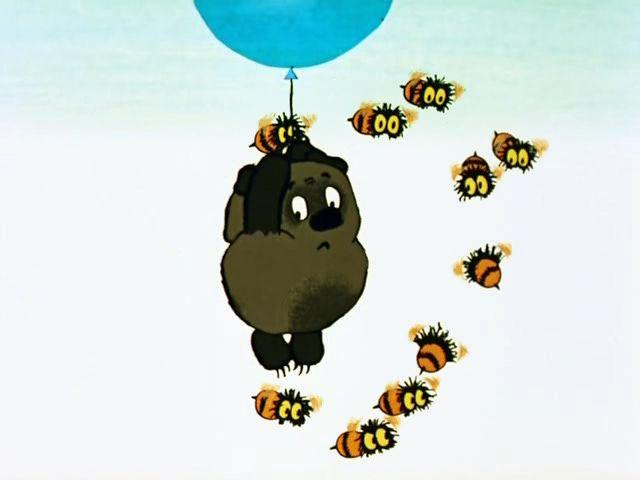
\includegraphics[width=9cm]{images/winnie_kr_4}
\end{figure}



\end{enumerate}


\subsection{Контрольная 4, решения}

\begin{enumerate}
\item[2.]
\begin{enumerate}
\item
\begin{align*}
  L(x, \lambda) &= \prod_{i=1}^{250} e^{-\lambda} \frac{\lambda^{x_i}}{x_i!} = e^{-250\lambda} \lambda^{\sum_{i=1}^{250} x_i} \prod_{i=1}^{250} \frac{1}{x_i!} \\
  l(x, \lambda) &= -250\lambda + \ln\lambda \sum_{i=1}^{250} x_i - \sum_{i=1}^{250} \ln x_i! \\
  \frac{\partial l}{\partial \lambda} &= -250 + \frac{1}{\lambda} \sum_{i=1}^{250} x_i \\
  \hat{\lambda}_{ML} &= \overline{X}
\end{align*}
\item $\E(\hat{\lambda}_{ML}) = \E(\overline{X}) = \lambda \Rightarrow$ оценка несмещённая.

$\Var(\hat{\lambda}_{ML}) = \Var(\overline{X}) = \frac{1}{n^2}\cdot n\Var(X_1) = \frac{\lambda}{n} \to_{n \to \infty} 0 \Rightarrow$ оценка состоятельная.

$\frac{\partial^2 l}{\partial \lambda^2} = -\frac{1}{\lambda^2} \sum_{i=1}^{n} x_i$, $I(\lambda) = - \E\left(-\frac{1}{\lambda^2} \sum_{i=1}^{n} x_i\right) = \frac{n}{\lambda}$.
Так как $\Var(\hat{\lambda}_{ML}) = \frac{1}{I(\lambda)}$, оценка является эффективной.
\item $\P(X=0) = \frac{\lambda^0 e^{-\lambda}}{0!} = e^{-\lambda} \Rightarrow \widehat{\P(X=0)} = e^{-\hat\lambda} = e^{-\overline{X}}$
\item В данном случае: $g(\hat{\lambda}) = e^{-\hat\lambda}$, $g'(\hat\lambda) = -e^{-\hat\lambda}$.
И доверительный интервал имеет вид:
\[
  \left[e^{-\overline{X}} - 1.96 \sqrt{\frac{e^{-2\overline{X}}\overline{X}}{n}}; e^{-\overline{X}} + 1.96 \sqrt{\frac{e^{-2\overline{X}}\overline{X}}{n}} \right]
\]
\end{enumerate}


\item[3.]
\begin{enumerate}
\item $\hat p \stackrel{as.}{\sim}\cN\left(p, \frac{p(1-p)}{n}\right)$

О1Р: лекарство помогает в $80\%$ случаев, но в данной выборке оно помогло менее чем 12 людям.

$\alpha = \P(\text{О1Р}) = \P\left(\hat p < \frac{12}{20} \vert p=0.8 \right) = \P \left(\frac{\hat p - 0.8}{\sqrt{\frac{0.8\cdot0.2}{20}}} < \frac{\frac{12}{20} - 0.8}{\sqrt{\frac{0.8\cdot0.2}{20}}} \right) = 0.0125$
\item О2Р: лекарство помогает в $60\%$ случаев, но $Y \geq 12$.

$\hat p \sim \cN\left(0.6, \frac{0.6\cdot0.4}{20} \right)$

$\beta = \P\left( \hat p \geq \frac{12}{20} \right) = \frac{1}{2}$
\item $\P(Z < a) =0.1$, из таблицы находим, что $a=-1.28$.
\[
a = \frac{\frac{c}{20} - 0.8}{\sqrt{\frac{0.8\cdot0.2}{20}}} = -1.28 \Rightarrow c \approx 13.7
\]
\item $\P(\vert \hat p - p \vert \leq 0.01) \geq 0.95$, будем считать, что $p=0.6$.
\[
\P(\vert \hat p - p \vert \leq 0.01) = \P(-0.01 \leq \hat p - p \leq 0.01) = \P\left(-\frac{0.01}{\sqrt{\frac{0.6\cdot0.4}{n}}} \leq Z \leq \frac{0.01}{\sqrt{\frac{0.6\cdot0.4}{n}}} \right) =0.95
\]
Из таблицы находим
\[
\frac{0.01}{\sqrt{\frac{0.6\cdot0.4}{n}}} = 1.96 \Rightarrow n = \frac{0.6\cdot0.4\cdot1.96^2}{0.01^2}
\]
\end{enumerate}

\item[4.] $H_0: p_{\text{c}} = \frac{1}{7}, p_{\text{л}} = \frac{2}{7}, p_{\text{к}} = \frac{4}{7}$

$Q = \sum_{i=1}^{s=3} \frac{(\nu_i - np_i)^2}{np_i} \sim \chi^2_{s-k-1} = \chi^2_2$

$Q_{obs} = \frac{\left(10-70\frac{1}{7}\right)^2}{70\frac{1}{7}} + \frac{\left(1-70\frac{2}{7}\right)^2}{70\frac{2}{7}} + \frac{\left(39-70\frac{4}{7}\right)^2}{70\frac{4}{7}} = 18.075$

$Q_{crit} = 5.99$, $Q_{crit} < Q_{obs} \Rightarrow$ гипотеза отвергается

\item[5.] $LR \sim \chi^2_1$, так как основная гипотеза содержит одно уравнение

$L(x, \lambda) = \prod_{i=1}^{n=50} \lambda e^{-\lambda x} = \lambda^{50} e^{-\lambda \sum_{i=1}^{n=50} x_i}$

$\ln L (x, \lambda) = 50\ln\lambda - \lambda \sum_{i=1}^{n=50} x_i \to \max_\lambda$

$\frac{\partial \ln L}{\partial \lambda} = \frac{50}{\lambda} - \sum_{i=1}^{n=50} x_i \mid_{\lambda=\hat{\lambda}} = 0 \Rightarrow \hat{\lambda}_{ML} = \frac{1}{\overline{X}} = \frac{10}{11}$

При верной $H_0:  \lambda=1$, тогда $\ln L (\lambda=1) = 50 \ln 1 - 1 \cdot 1.1 \cdot 50 = -55$

При верной $H_1: \lambda=\lambda_{ML}$, тогда $\ln L \left(\lambda=\frac{10}{11}\right) = 50 \ln \frac{10}{11} - \frac{10}{11} \cdot 50 \cdot 1.1 = -54.77$

$LR_{obs} = 2(\ln L (H_1) - \ln(H_0)) = 2(-54.77- (-55)) = 0.46$

$LR_{crit} = 2.71$, $LR_{crit} > LR_{obs} \Rightarrow$ оснований отвергать $H_0$ нет

\item[6.]  Будем проверять гипотезы на уровне значимости $0.05$
\begin{enumerate}
\item $\hat{\sigma}^2_{\text{в}} = 484$, $\hat{\sigma}^2_{\text{р}} = 400$

$\frac{\hat{\sigma}^2_{\text{в}} }{\hat{\sigma}^2_{\text{р}}} \sim F_{21-1 , 19-1}$

$F_{obs} = \frac{484}{400} = 1.21$, $F_{crit, left} = 0.4$, $F_{crit, right} = 2.6  \Rightarrow$ оснований отвергать $H_0$ нет

\item $\hat{\sigma}_0^2 = \frac{22\cdot (21-1) + 20 \cdot (19-1)}{21 + 19 - 2} \approx 21$

$t_{obs} = \frac{78-67}{\sqrt{21} \sqrt{\frac{1}{21}+ \frac{1}{21}}} \approx 7.8 $

$t_{crit}  \sim t_{21+19-2} = t_{38}$, $t_{crit} = \pm 2.02 \Rightarrow$ гипотеза отвергается
\end{enumerate}
\item[7.] $\gamma = \sum_{i=1}^s \sum_{j=1}^m \frac{\left(n_{ij} - \frac{n_{i\cdot}n_{\cdot j}}{n}\right)^2}{\frac{n_{i\cdot}n_{\cdot j}}{n}} \sim \chi^2_{(s-1)(m-1)}$

$\gamma_{obs} = \frac{\left(12-\frac{44\cdot48}{100}\right)^2}{\frac{44\cdot48}{100}} + \frac{\left(36-\frac{56\cdot48}{100}\right)^2}{\frac{56\cdot48}{100}} + \frac{\left(32-\frac{44\cdot52}{100}\right)^2}{\frac{44\cdot52}{100}} + \frac{\left(20-\frac{50\cdot52}{100}\right)^2}{\frac{50\cdot52}{100}} \approx 12$

$\gamma_{crit} = 3.84 \Rightarrow$  гипотеза отвергается

\end{enumerate}


\subsection{Экзамен, 20.06.2016}

\element{prob_one_sample}{ % в фигурных скобках название группы вопросов
 \AMCcompleteMulti
  \begin{questionmult}{1} % тип вопроса (questionmult --- множественный выбор) и в фигурных --- номер вопроса
  Случайные величины $X$ и $Y$ распределены нормально. Для тестирования гипотезы о равенстве дисперсий выбирается $m$ наблюдений случайной величины $X$ и $n$ наблюдений случайной величины $Y$. Какое распределение может иметь статистика, используемая в данном случае?
 \begin{multicols}{3} % располагаем ответы в 3 колонки
   \begin{choices} % опция [o] не рандомизирует порядок ответов
      \correctchoice{$F_{m-1,n-1}$}
      \wrongchoice{$F_{m+1,n+1}$}
      \wrongchoice{$F_{m,n}$}
      \wrongchoice{$t_{m+n-2}$}
      \wrongchoice{$t_{m+n-1}$}
      \end{choices}
  \end{multicols}
  \end{questionmult}
}

\element{prob_one_sample}{ % в фигурных скобках название группы вопросов
 \AMCcompleteMulti
  \begin{questionmult}{2} % тип вопроса (questionmult --- множественный выбор) и в фигурных --- номер вопроса
  Требуется проверить гипотезу о равенстве математических ожиданий в двух нормальных выборках размером $m$ и $n$. Если дисперсии неизвестны, но равны, то тестовая статистика имеет распределение
 \begin{multicols}{3} % располагаем ответы в 3 колонки
   \begin{choices} % опция [o] не рандомизирует порядок ответов
      \correctchoice{$t_{m+n-2}$}
      \wrongchoice{$F_{m+1,n+1}$}
      \wrongchoice{$F_{m,n}$}
      \wrongchoice{$F_{m-1,n-1}$}
      \wrongchoice{$t_{m+n-1}$}
      \end{choices}
  \end{multicols}
  \end{questionmult}
}


\element{prob_one_sample}{ % в фигурных скобках название группы вопросов
 \AMCcompleteMulti
  \begin{questionmult}{3} % тип вопроса (questionmult --- множественный выбор) и в фигурных --- номер вопроса
  Требуется проверить гипотезу о равенстве дисперсий по двум нормальным выборкам размером $20$ и $16$ наблюдений. Несмещённая оценка дисперсии по первой выборке составила $60$, по второй — $90$. Тестовая статистика может быть равна
 \begin{multicols}{3} % располагаем ответы в 3 колонки
   \begin{choices} % опция [o] не рандомизирует порядок ответов
      \correctchoice{$1.5$}
      \wrongchoice{$1$}
      \wrongchoice{$1.224$}
      \wrongchoice{$2$}
      \wrongchoice{$4$}
      \end{choices}
  \end{multicols}
  \end{questionmult}
}


\element{prob_one_sample}{ % в фигурных скобках название группы вопросов
 \AMCcompleteMulti
  \begin{questionmult}{4} % тип вопроса (questionmult --- множественный выбор) и в фигурных --- номер вопроса
  Требуется проверить гипотезу о равенстве математических ожиданий по двум нормальным выборкам размером $20$ и $16$ наблюдений. Истинные дисперсии по обеим выборкам известны, совпадают и равны $16$. Разница выборочных средних равна $1$. Тестовая статистика может быть равна
 \begin{multicols}{3} % располагаем ответы в 3 колонки
   \begin{choices} % опция [o] не рандомизирует порядок ответов
      \wrongchoice{$1.5$}
      \wrongchoice{$1$}
      \wrongchoice{$1.224$}
      \wrongchoice{$2$}
      \wrongchoice{$4$}
      \end{choices}
  \end{multicols}
  \end{questionmult}
}


\element{prob_one_sample}{ % в фигурных скобках название группы вопросов
 \AMCcompleteMulti
  \begin{questionmult}{5} % тип вопроса (questionmult --- множественный выбор) и в фигурных --- номер вопроса
  При проверке гипотезе о равенстве математических ожиданий в двух нормальных выборках размеров $m$ и $n$ при известных, но не равных дисперсиях, тестовая статистика имеет распределение
 \begin{multicols}{3} % располагаем ответы в 3 колонки
   \begin{choices} % опция [o] не рандомизирует порядок ответов
      \correctchoice{$N(0;1)$}
      \wrongchoice{$F_{m-1,n-1}$}
      \wrongchoice{$F_{m}$}
      \wrongchoice{$t_{m+n-2}$}
      \wrongchoice{$t_{m+n-1}$}
      \end{choices}
  \end{multicols}
  \end{questionmult}
}


\element{prob_one_sample}{ % в фигурных скобках название группы вопросов
 \AMCcompleteMulti
  \begin{questionmult}{6} % тип вопроса (questionmult --- множественный выбор) и в фигурных --- номер вопроса
  При проверке гипотезы о равенстве долей используется следующее распределение
 \begin{multicols}{3} % располагаем ответы в 3 колонки
   \begin{choices} % опция [o] не рандомизирует порядок ответов
      \correctchoice{$N(0;1)$}
      \wrongchoice{$F_{m-1,n-1}$}
      \wrongchoice{$F_{m, n}$}
      \wrongchoice{$t_{m+n-2}$}
      \wrongchoice{$t_{m+n-1}$}
      \end{choices}
  \end{multicols}
  \end{questionmult}
}


\element{prob_one_sample_rejected}{ % в фигурных скобках название группы вопросов
 \AMCcompleteMulti
  \begin{questionmult}{7} % тип вопроса (questionmult --- множественный выбор) и в фигурных --- номер вопроса
   Есть две нормально распределённых выборки размером $20$ и $16$ наблюдений. Истинные дисперсии по обеим выборкам неизвестны и равны. Выборочные средние по обеим выборкам совпадают. Гипотеза о равенстве математических ожиданий
 %\begin{multicols}{3} % располагаем ответы в 3 колонки
   \begin{choices} % опция [o] не рандомизирует порядок ответов
      \correctchoice{не отвергается на любом разумном уровне значимости}
      \wrongchoice{отвергается на любом разумном уровне значимости}
      \wrongchoice{не отвергается на 5\%-ом и отвергается на 1\%-ом уровне значимости}
      \wrongchoice{не отвергается на 1\%-ом и отвергается на 5\%-ом уровне значимости}
      \wrongchoice{Гипотезу невозможно проверить}
      \end{choices}
  %\end{multicols}
  \end{questionmult}
}


\element{prob_one_sample}{ % в фигурных скобках название группы вопросов
 \AMCcompleteMulti
  \begin{questionmult}{8} % тип вопроса (questionmult --- множественный выбор) и в фигурных --- номер вопроса
  Для проверки гипотезы о равенстве долей в двух выборках  могут использоваться следующие распределения
 \begin{multicols}{3} % располагаем ответы в 3 колонки
   \begin{choices} % опция [o] не рандомизирует порядок ответов
      \wrongchoice{только $N(0;1)$}
      \correctchoice{$N(0;1)$ и $\chi^2_1$}
      \wrongchoice{только $\chi^2_1$}
      \wrongchoice{$N(0;1)$ и $F_{m,n}$}
      \wrongchoice{только $F_{m,n}$}
      \end{choices}
  \end{multicols}
  \end{questionmult}
}

\element{prob_one_sample}{ % в фигурных скобках название группы вопросов
 \AMCcompleteMulti
  \begin{questionmult}{9} % тип вопроса (questionmult --- множественный выбор) и в фигурных --- номер вопроса
  Доля успехов в первой выборке равна $0.55$, доля успехов во второй выборке --- $0.4$. Количество наблюдений в выборках равно $40$ и $20$ соответственно. Тестовая статистика для проверки гипотезы о равенстве долей может быть равна
 \begin{multicols}{3} % располагаем ответы в 3 колонки
   \begin{choices} % опция [o] не рандомизирует порядок ответов
      \correctchoice{$1.1$}
      \wrongchoice{$2.2$}
      \wrongchoice{$1.2$}
      \wrongchoice{$2.4$}
      \wrongchoice{$0.9$}
      \end{choices}
  \end{multicols}
  \end{questionmult}
}

\element{prob_one_sample}{ % в фигурных скобках название группы вопросов
 \AMCcompleteMulti
  \begin{questionmult}{10} % тип вопроса (questionmult --- множественный выбор) и в фигурных --- номер вопроса
  Доля успехов в первой выборке равна $0.8$, доля успехов во второй выборке --- $0.3$. Количество наблюдений в выборках $40$ и $20$ соответственно. Гипотеза о равенстве долей
 %\begin{multicols}{3} % располагаем ответы в 3 колонки
   \begin{choices} % опция [o] не рандомизирует порядок ответов
     \correctchoice{отвергается на любом разумном уровне значимости}
     \wrongchoice{не отвергается на любом разумном уровне значимости}
     \wrongchoice{не отвергается на 5\%-ом и отвергается на 1\%-ом уровне значимости}
     \wrongchoice{не отвергается на 1\%-ом и отвергается на 5\%-ом уровне значимости}
     \wrongchoice{Гипотезу невозможно проверить}
      \end{choices}
  %\end{multicols}
  \end{questionmult}
}























\element{prob_two_samples}{ % в фигурных скобках название группы вопросов
 \AMCcompleteMulti
  \begin{questionmult}{2} % тип вопроса (questionmult --- множественный выбор) и в фигурных --- номер вопроса
  Для выборки $X_1,\ldots,X_n$, имеющей нормальное распределение, проверяется гипотеза $H_0: \sigma^2=\sigma_0^2$ против $H_a: \sigma^2 > \sigma_0^2$. Критическая область имеет вид
 %\begin{multicols}{3} % располагаем ответы в 3 колонки
   \begin{choices} % опция [o] не рандомизирует порядок ответов
      \correctchoice{$(A,+\infty)$, где $A$ таково, что $\P(\chi^2_{n-1} < A) =1-\alpha$}
      \wrongchoice{$(A,+\infty)$, где $A$ таково, что $\P(\chi^2_{n-1} < A)  =\alpha$}
      \wrongchoice{$(0,A)$, где $A$ таково, что $\P(\chi^2_{n-1} < A)  =1-\alpha$}
      \wrongchoice{$(-\infty,A)$, где $A$ таково, что $\P(\chi^2_{n-1} < A)  =1-\alpha$}
      \wrongchoice{ $(0,A)$, где $A$ таково, что $\P(\chi^2_{n-1} < A)  =\alpha$}
      \end{choices}
  %\end{multicols}
  \end{questionmult}
}


% \element{prob_two_samples_rejected}{ % в фигурных скобках название группы вопросов
%  \AMCcompleteMulti
%   \begin{questionmult}{3} % тип вопроса (questionmult --- множественный выбор) и в фигурных --- номер вопроса
%   Для выборки $X_1,\ldots,X_n$, имеющей нормальное распределение, проверяется гипотеза $H_0: \sigma^2=\sigma_0^2$ против $H_a: \sigma^2 < \sigma_0^2$. Критическая область имеет вид
%  %\begin{multicols}{3} % располагаем ответы в 3 колонки
%    \begin{choices} % опция [o] не рандомизирует порядок ответов
%       \correctchoice{$(0,A)$, где $A$ таково, что $F_{\chi^2_{n-1}} (A) =\alpha$}
%       \wrongchoice{$(0,A)$, где $A$ таково, что $F_{\chi^2_{n-1}} (A) =1-\alpha$}
%       \wrongchoice{$(-\infty,A)$, где $A$ таково, что $F_{\chi^2_{n-1}} (A) =\alpha$}
%       \wrongchoice{ $(A,+\infty)$, где $A$ таково, что $F_{\chi^2_{n-1}} (A) =1-\alpha$}
%       \end{choices}
%   %\end{multicols}
%   \end{questionmult}
% }


\element{prob_two_samples}{ % в фигурных скобках название группы вопросов
 \AMCcompleteMulti
  \begin{questionmult}{4} % тип вопроса (questionmult --- множественный выбор) и в фигурных --- номер вопроса
  При подбрасывании игральной кости 600 раз шестерка выпала 105 раз. Гипотеза о том, что кость правильная
 %\begin{multicols}{3} % располагаем ответы в 3 колонки
   \begin{choices} % опция [o] не рандомизирует порядок ответов
      \correctchoice{не отвергается при любом разумном значении $\alpha$}
      \wrongchoice{отвергается при любом разумном значении $\alpha$}
      \wrongchoice{отвергается при $\alpha = 0.05$, не отвергается при $\alpha = 0.01$}
      \wrongchoice{отвергается при $\alpha = 0.01$, не отвергается при $\alpha = 0.05$}
      \wrongchoice{Гипотезу невозможно проверить}
      \end{choices}
  %\end{multicols}
  \end{questionmult}
}


\element{prob_two_samples}{ % в фигурных скобках название группы вопросов
 \AMCcompleteMulti
  \begin{questionmult}{5} % тип вопроса (questionmult --- множественный выбор) и в фигурных --- номер вопроса
  Величины $X_1,\ldots,X_n$ --- выборка из нормально распределенной случайной величины с неизвестным математическим ожиданием и известной дисперсией. На уровне значимости $\alpha$ проверяется гипотеза $H_0: \mu = \mu_0$ против $H_a: \mu \neq \mu_0$. Обозначим $\varphi_1$ и $\varphi_2$ вероятности ошибок первого и второго рода соответственно. Между параметрами задачи всегда выполнено соотношение
 \begin{multicols}{3} % располагаем ответы в 3 колонки
   \begin{choices} % опция [o] не рандомизирует порядок ответов
      \correctchoice{$\varphi_1 = \alpha$}
      \wrongchoice{$\varphi_1 = 1 - \alpha$}
      \wrongchoice{$\varphi_2 = \alpha$}
      \wrongchoice{$\varphi_2 = 1 - \alpha$}
      \wrongchoice{$\varphi_1 + \varphi_2 = \alpha$}
      \end{choices}
  \end{multicols}
  \end{questionmult}
}


\element{prob_two_samples}{ % в фигурных скобках название группы вопросов
 \AMCcompleteMulti
  \begin{questionmult}{6} % тип вопроса (questionmult --- множественный выбор) и в фигурных --- номер вопроса
  По случайной выборке из 200 наблюдений было оценено выборочное среднее $\bar{X} = 25$  и несмещённая оценка дисперсии $\hat{\sigma}^2 = 25$. В рамках проверки гипотезы $H_0: \mu = 20$ против $H_a: \mu > 20$ можно сделать вывод, что гипотеза $H_0$
 %\begin{multicols}{3} % располагаем ответы в 3 колонки
   \begin{choices} % опция [o] не рандомизирует порядок ответов
      \correctchoice{отвергается при любом разумном значении $\alpha$}
      \wrongchoice{отвергается при $\alpha = 0.05$, не отвергается при $\alpha = 0.01$}
      \wrongchoice{отвергается при $\alpha = 0.01$, не отвергается при $\alpha = 0.05$}
      \wrongchoice{не отвергается при любом разумном значении $\alpha$}
      \wrongchoice{Гипотезу невозможно проверить}
      \end{choices}
  %\end{multicols}
  \end{questionmult}
}


\element{prob_two_samples}{ % в фигурных скобках название группы вопросов
 \AMCcompleteMulti
  \begin{questionmult}{7} % тип вопроса (questionmult --- множественный выбор) и в фигурных --- номер вопроса
   По выборке $X_1,\ldots, X_n$ из нормального распределения строятся по стандартным формулам доверительные интервалы для математического ожидания. Получен интервал $(a_1,a_2)$ при известной дисперсии и интервал $(b_1,b_2)$ при неизвестной дисперсии. Всегда справедливы следующие соотношения:
 \begin{multicols}{2} % располагаем ответы в 3 колонки
   \begin{choices} % опция [o] не рандомизирует порядок ответов
      \correctchoice{$|a_1-b_1| = |a_2-b_2|$}
      \wrongchoice{$a_2 - a_1 < b_2 - b_1$}
      \wrongchoice{$a_2 - a_1 > b_2 - b_1$}
      \wrongchoice{$a_1<0,b_1<0,a_2>0,b_2>0$}
      \wrongchoice{$a_1>0,b_1>0,a_2>0,b_2>0$}
      \end{choices}
  \end{multicols}
  \end{questionmult}
}


\element{prob_two_samples}{ % в фигурных скобках название группы вопросов
 \AMCcompleteMulti
  \begin{questionmult}{8} % тип вопроса (questionmult --- множественный выбор) и в фигурных --- номер вопроса
  Величины $X_1,\ldots,X_n$ --- выборка из нормального распределения.  Статистика $U=\frac{5-\bar{X}}{5/\sqrt{n}}$ применима для проверки
 %\begin{multicols}{3} % располагаем ответы в 3 колонки
   \begin{choices} % опция [o] не рандомизирует порядок ответов
      \wrongchoice{гипотезы $H_0: \mu = 5$ при известной дисперсии, равной 5, при любых $n$}
      \correctchoice{гипотезы $H_0: \mu = 5$ при известной дисперсии, равной 25, при любых $n$}
      \wrongchoice{гипотезы $H_0: \mu = 5$ при известной дисперсии, равной 5, при больших $n$}
      \wrongchoice{гипотезы $H_0: \mu = 5$ при известной дисперсии, равной 25, только при больших $n$}
      \wrongchoice{гипотезы $H_0: \sigma = 5$}
      \end{choices}
  %\end{multicols}
  \end{questionmult}
}

\element{prob_two_samples}{ % в фигурных скобках название группы вопросов
 \AMCcompleteMulti
  \begin{questionmult}{9} % тип вопроса (questionmult --- множественный выбор) и в фигурных --- номер вопроса
Выборочная доля успехов в некотором испытании составляет $0.3$. Исследователь Ромео хочет, чтобы длина двустороннего 95\%-го доверительного интервала для истинной доли не превышала $0.1$. Количество наблюдений, необходимых для этого, примерно равно
 \begin{multicols}{3} % располагаем ответы в 3 колонки
   \begin{choices} % опция [o] не рандомизирует порядок ответов
      \correctchoice{$322$}
      \wrongchoice{$161$}
      \wrongchoice{$113$}
      \wrongchoice{$225$}
      \wrongchoice{$81$}
      \end{choices}
  \end{multicols}
  \end{questionmult}
}

\element{prob_two_samples}{ % в фигурных скобках название группы вопросов
 \AMCcompleteMulti
  \begin{questionmult}{10} % тип вопроса (questionmult --- множественный выбор) и в фигурных --- номер вопроса
  Пусть $X_1,\ldots,X_n$ --- выборка из нормального распределения с известной дисперсией $\sigma^2$. Пусть $U = \frac{\bar{X}-\mu_0}{\sigma/\sqrt{n}}$. Величина $U^2$ имеет распределение
 \begin{multicols}{3} % располагаем ответы в 3 колонки
   \begin{choices} % опция [o] не рандомизирует порядок ответов
     \correctchoice{$\chi^2_1$}
     \wrongchoice{$\chi^2_{n-1}$}
     \wrongchoice{$t_1$}
     \wrongchoice{$t_{n-1}$}
     \wrongchoice{$F_{1,n-1}$}
      \end{choices}
  \end{multicols}
  \end{questionmult}
}
























\element{prob_sample_char}{ % в фигурных скобках название группы вопросов
 \AMCcompleteMulti
  \begin{questionmult}{1} % тип вопроса (questionmult --- множественный выбор) и в фигурных --- номер вопроса
  Дана реализация выборки: 3, 1, 2. Выборочный начальный момент первого порядка равен
 \begin{multicols}{3} % располагаем ответы в 3 колонки
   \begin{choices} % опция [o] не рандомизирует порядок ответов
      \correctchoice{2}
      \wrongchoice{1}
      \wrongchoice{0}
      \wrongchoice{3}
      \wrongchoice{14/3}
      \end{choices}
  \end{multicols}
  \end{questionmult}
}

\element{prob_sample_char}{ % в фигурных скобках название группы вопросов
 \AMCcompleteMulti
  \begin{questionmult}{2} % тип вопроса (questionmult --- множественный выбор) и в фигурных --- номер вопроса
  Дана реализация выборки: 3, 1, 2. Несмещённая оценка дисперсии равна
 \begin{multicols}{3} % располагаем ответы в 3 колонки
   \begin{choices} % опция [o] не рандомизирует порядок ответов
      \correctchoice{1}
      \wrongchoice{1/2}
      \wrongchoice{1/3}
      \wrongchoice{2/3}
      \wrongchoice{2}
      \end{choices}
  \end{multicols}
  \end{questionmult}
}


\element{prob_sample_char}{ % в фигурных скобках название группы вопросов
 \AMCnoCompleteMulti
  \begin{questionmult}{3} % тип вопроса (questionmult --- множественный выбор) и в фигурных --- номер вопроса
  Выберите НЕВЕРНОЕ утверждение про эмпирическую функцию распределения $F_n(x)$
 %\begin{multicols}{3} % располагаем ответы в 3 колонки
   \begin{choices} % опция [o] не рандомизирует порядок ответов
      \correctchoice{$F_n(x)$ является невозрастающей функцией}
      %\wrongchoice{$F_n(x)$ является состоятельной оценкой функции распределения $F(x)$}
      \wrongchoice{$F_n(x)$ имеет разрыв в каждой точке вариационного ряда}
      \wrongchoice{$F_n(x)$ асимптотически нормальна}
      \wrongchoice{$\E(F_n(x))=F(x)$}
      \wrongchoice{$\Var(F_n(x))=F(x)(1-F(x))/n$}
      \end{choices}
  %\end{multicols}
  \end{questionmult}
}


\element{prob_sample_char}{ % в фигурных скобках название группы вопросов
 \AMCcompleteMulti
  \begin{questionmult}{4} % тип вопроса (questionmult --- множественный выбор) и в фигурных --- номер вопроса
 Юрий Петров утверждает, что обычно посещает половину занятий по Статистике. За последние полгода из 36 занятий он не посетил ни одного. Вычислите значение критерия хи-квадрат Пирсона для гипотезы, что утверждение Юрия Петрова истинно и укажите число степеней свободы
 \begin{multicols}{3} % располагаем ответы в 3 колонки
   \begin{choices} % опция [o] не рандомизирует порядок ответов
      \correctchoice{$\chi^2 = 36$, $df=1$}
      \wrongchoice{$\chi^2 = 2$, $df=2$}
      \wrongchoice{$\chi^2 = 14$, $df=1$}
      \wrongchoice{$\chi^2 = 20$, $df=2$}
      \wrongchoice{$\chi^2 = 24$, $df=1$}
      \end{choices}
  \end{multicols}
  \end{questionmult}
}


\element{prob_sample_char}{ % в фигурных скобках название группы вопросов
 \AMCcompleteMulti
  \begin{questionmult}{5} % тип вопроса (questionmult --- множественный выбор) и в фигурных --- номер вопроса
  Производитель фломастеров попросил трёх человек оценить два вида фломастеров: «Лесенка» и «Erich Krause» по 10-балльной шкале:

\begin{center}
\begin{tabular}{lrrr} \toprule
 & Пафнутий & Андрей & Карл \\
\midrule
Лесенка & 9 & 7 & 6 \\
Erich Krause & 8 & 9 & 7 \\
\bottomrule
\end{tabular}
\end{center}

\textbf{Точное} $P$-значение ($P$-value) статистики теста знаков равно

 \begin{multicols}{3} % располагаем ответы в 3 колонки
   \begin{choices} % опция [o] не рандомизирует порядок ответов
      \correctchoice{1/2}
      \wrongchoice{1/8}
      \wrongchoice{1/3}
      \wrongchoice{3/8}
      \wrongchoice{2/3}
      \end{choices}
  \end{multicols}
  \end{questionmult}
}


\element{prob_sample_char}{ % в фигурных скобках название группы вопросов
 \AMCcompleteMulti
  \begin{questionmult}{6} % тип вопроса (questionmult --- множественный выбор) и в фигурных --- номер вопроса
  Производитель фломастеров попросил трёх человек оценить два вида фломастеров: «Лесенка» и «Erich Krause» по 10-балльной шкале:

\begin{center}
\begin{tabular}{lrrr} \toprule
 & Пафнутий  & Андрей & Карл \\
\midrule
Лесенка & 9 & 7 & 6 \\
Erich Krause & 8 & 9 & 7 \\
\bottomrule
\end{tabular}
\end{center}

Вычислите модуль значения статистики теста знаков. \textbf{Используя нормальную аппроксимацию}, проверьте на уровне значимости 0.1 гипотезу о том, что фломастеры имеют одинаковое качество.

 \begin{multicols}{3} % располагаем ответы в 3 колонки
   \begin{choices} % опция [o] не рандомизирует порядок ответов
      \correctchoice{0.58, $H_0$ не отвергается}
      \wrongchoice{0.58, $H_0$ отвергается}
      \wrongchoice{0.43, $H_0$ не отвергается}
      \wrongchoice{1.65, $H_0$ отвергается}
      \wrongchoice{1.96, $H_0$ отвергается}
      \end{choices}
  \end{multicols}
  \end{questionmult}
}


\element{prob_sample_char}{ % в фигурных скобках название группы вопросов
 \AMCcompleteMulti
  \begin{questionmult}{7} % тип вопроса (questionmult --- множественный выбор) и в фигурных --- номер вопроса
   Кузнец Вакула в течение 100 лет ведет статистику о прилете аистов и рождении младенцев на хуторе близ Диканьки. У него получилась следующая таблица сопряженности

\begin{center}
\begin{tabular}{lrr} \toprule
& Аисты прилетали  & Аисты не прилетали \\
\midrule
Появлялся младенец & 30 & 10 \\
Не появлялся младенец & 30 & 30 \\
\bottomrule
\end{tabular}
\end{center}

Укажите число степеней свободы статистики Пирсона и на уровне значимости 5\% определите, зависит ли появление младенца от прилета аистов

 \begin{multicols}{3} % располагаем ответы в 3 колонки
   \begin{choices} % опция [o] не рандомизирует порядок ответов
      \correctchoice{$df=1$, зависит}
      \wrongchoice{$df=1$, не зависит}
      \wrongchoice{$df=3$, зависит}
      \wrongchoice{$df=4$, зависит}
      \wrongchoice{$df=2$, зависит}
      \end{choices}
  \end{multicols}
  \end{questionmult}
}



\element{prob_sample_char}{ % в фигурных скобках название группы вопросов
 \AMCcompleteMulti
  \begin{questionmult}{8} % тип вопроса (questionmult --- множественный выбор) и в фигурных --- номер вопроса
  В коробке 50 купюр пяти различных номиналов. Случайным образом достаются две купюры. Номиналы вынимаемых купюр
 \begin{multicols}{2} % располагаем ответы в 3 колонки
   \begin{choices} % опция [o] не рандомизирует порядок ответов
   \correctchoice{отрицательно коррелированы}
   \wrongchoice{положительно коррелированы}
    \wrongchoice{не коррелированы и не зависимы}
    \wrongchoice{не коррелированы, но зависимы}
    \wrongchoice{положительно коррелированы, но не зависимы}
      \end{choices}
  \end{multicols}
  \end{questionmult}
}



\element{prob_sample_char}{ % в фигурных скобках название группы вопросов
 \AMCcompleteMulti
  \begin{questionmult}{9} % тип вопроса (questionmult --- множественный выбор) и в фигурных --- номер вопроса
Экзамен принимают два преподавателя: Злой и Добрый. Они поставили следующие оценки:

\begin{center}
\begin{tabular}{lrrrrr} \toprule
Злой   & 2 & 3 & 10 & 8 & 3 \\
Добрый & 6 & 4 & 7  & 8 & \\
\bottomrule
\end{tabular}
\end{center}

Значение статистики критерия Вилкоксона о совпадении распределений оценок равно

 \begin{multicols}{3} % располагаем ответы в 3 колонки
   \begin{choices} % опция [o] не рандомизирует порядок ответов
     \correctchoice{22.5}
     \wrongchoice{7.5}
     \wrongchoice{19}
     \wrongchoice{20}
     \wrongchoice{20.5}
      \end{choices}
  \end{multicols}
  \end{questionmult}
}



\element{prob_sample_char}{ % в фигурных скобках название группы вопросов
 \AMCcompleteMulti
  \begin{questionmult}{10} % тип вопроса (questionmult --- множественный выбор) и в фигурных --- номер вопроса
Датчик случайных чисел выдал два значения псевдослучайных чисел: $0.5$ и $0.9$. Вычислите значение критерия Колмогорова и проверьте гипотезу о соответствии распределения равномерному на уровне значимости $0.1$. Критическое значение статистики Колмогорова для уровня значимости $0.1$ и двух наблюдений равно $0.776$.
 \begin{multicols}{3} % располагаем ответы в 3 колонки
   \begin{choices} % опция [o] не рандомизирует порядок ответов
      \correctchoice{$0.5$, $H_0$ не отвергается}
      \wrongchoice{$1.4$, $H_0$ отвергается}
      \wrongchoice{$0.9$, $H_0$ отвергается}
      \wrongchoice{$0.9$, $H_0$ не отвергается}
      \wrongchoice{$0.4$, $H_0$ не отвергается}
      \end{choices}
  \end{multicols}
  \end{questionmult}
}


























\element{prob_ml_mm}{ % в фигурных скобках название группы вопросов
 \AMCnoCompleteMulti
  \begin{questionmult}{1} % тип вопроса (questionmult --- множественный выбор) и в фигурных --- номер вопроса
  Выберите НЕВЕРНОЕ утверждение про метод максимального правдоподобия (ММП):
 %\begin{multicols}{3} % располагаем ответы в 3 колонки
   \begin{choices} % опция [o] не рандомизирует порядок ответов
      \correctchoice{Оценки ММП асимтотически нормальны $\cN(0;1)$}
      \wrongchoice{ММП применим для зависимых случайных величин}
      \wrongchoice{ММП применим для оценивания двух и более параметров}
      \wrongchoice{При выполнении технических предпосылок оценки ММП состоятельны}
      \wrongchoice{ММП оценки не всегда совпадают с оценками метода моментов}
      \end{choices}
  %\end{multicols}
  \end{questionmult}
}

\element{prob_ml_mm}{ % в фигурных скобках название группы вопросов
 \AMCcompleteMulti
  \begin{questionmult}{2} % тип вопроса (questionmult --- множественный выбор) и в фигурных --- номер вопроса
  Если величина $\hat\theta$ имеет нормальное распределение $\cN(2;0.01^2)$, то, согласно дельта-методу, $\hat\theta^2$ имеет примерно нормальное распределение
 \begin{multicols}{3} % располагаем ответы в 3 колонки
   \begin{choices} % опция [o] не рандомизирует порядок ответов
      \correctchoice{$\cN(4;16\cdot 0.01^2)$}
      \wrongchoice{$\cN(4;4\cdot 0.01^2)$}
      \wrongchoice{$\cN(2;4\cdot 0.01^2)$}
      \wrongchoice{$\cN(4;8\cdot 0.01^2)$}
      \wrongchoice{$\cN(4;2\cdot 0.01^2)$}
      \end{choices}
  \end{multicols}
  \end{questionmult}
}


\element{prob_ml_mm}{ % в фигурных скобках название группы вопросов
 \AMCcompleteMulti
  \begin{questionmult}{3} % тип вопроса (questionmult --- множественный выбор) и в фигурных --- номер вопроса
  Случайные величины $X_1$, $X_2$ и $X_3$ независимы и одинаково распределены,

\begin{center}
  \begin{tabular}{lrr} \toprule
  $X_i$ & 3 & 5 \\
  \midrule
  $\P(\cdot)$ & $p$ & $1-p$ \\
  \bottomrule
  \end{tabular}
\end{center}

  Имеется выборка из трёх наблюдений: $X_1=5$, $X_2=3$, $X_3=5$. Оценка неизвестного $p$, полученная методом максимального правдоподобия, равна:


 \begin{multicols}{3} % располагаем ответы в 3 колонки
   \begin{choices} % опция [o] не рандомизирует порядок ответов
      \correctchoice{$1/3$}
      \wrongchoice{$1/2$}
      \wrongchoice{$1/4$}
      \wrongchoice{$2/3$}
      \wrongchoice{Метод неприменим}
      \end{choices}
  \end{multicols}
  \end{questionmult}
}


\element{prob_ml_mm}{ % в фигурных скобках название группы вопросов
 \AMCcompleteMulti
  \begin{questionmult}{4} % тип вопроса (questionmult --- множественный выбор) и в фигурных --- номер вопроса
    Случайные величины $X_1$, $X_2$ и $X_3$ независимы и одинаково распределены,

\begin{center}
    \begin{tabular}{lrr} \toprule
    $X_i$ & 3 & 5 \\
    \midrule
    $\P(\cdot)$ & $p$ & $1-p$ \\
    \bottomrule
    \end{tabular}
\end{center}

    По выборке оказалось, что $\bar X = 4.5$. Оценка неизвестного $p$, полученная методом моментов, равна:


   \begin{multicols}{3} % располагаем ответы в 3 колонки
     \begin{choices} % опция [o] не рандомизирует порядок ответов
        \correctchoice{$1/4$}
        \wrongchoice{$1/2$}
        \wrongchoice{$1/3$}
        \wrongchoice{$2/3$}
        \wrongchoice{Метод неприменим}
      \end{choices}
  \end{multicols}
  \end{questionmult}
}

\element{prob_ml_mm}{ % в фигурных скобках название группы вопросов
 \AMCcompleteMulti
  \begin{questionmult}{5} % тип вопроса (questionmult --- множественный выбор) и в фигурных --- номер вопроса
  Величины $X_1$, $X_2$, \ldots, $X_{2016}$ независимы и одинаково распределены, $\cN(\mu ; 42)$. Оказалось, что $\bar X =  -23$. Про оценки метода моментов, $\hat \mu_{MM}$, и метода максимального правдоподобия, $\hat \mu_{ML}$, можно утверждать, что

 \begin{multicols}{3} % располагаем ответы в 3 колонки
   \begin{choices} % опция [o] не рандомизирует порядок ответов
      \correctchoice{$\hat \mu_{ML} = -23$, $\hat\mu_{MM} = -23$}
      \wrongchoice{$\hat \mu_{ML} > -23$, $\hat\mu_{MM} = -23$}
      \wrongchoice{$\hat \mu_{ML} = -23$, $\hat\mu_{MM} > -23$}
      \wrongchoice{$\hat \mu_{ML} < -23$, $\hat\mu_{MM} = -23$}
      \wrongchoice{$\hat \mu_{ML} = -23$, $\hat\mu_{MM} < -23$}
      \end{choices}
  \end{multicols}
  \end{questionmult}
}


\element{prob_ml_mm}{ % в фигурных скобках название группы вопросов
 \AMCnoCompleteMulti
  \begin{questionmult}{6} % тип вопроса (questionmult --- множественный выбор) и в фигурных --- номер вопроса
 Выберите НЕВЕРНОЕ утверждение про логарифмическую функцию правдоподобия $\ell(\theta)$

 %\begin{multicols}{3} % располагаем ответы в 3 колонки
   \begin{choices} % опция [o] не рандомизирует порядок ответов
      \correctchoice{Функция $\ell(\theta)$ имеет максимум при $\theta=0$}
      \wrongchoice{Функция $\ell(\theta)$ может принимать отрицательные значения}
      \wrongchoice{Функция $\ell(\theta)$ может принимать положительные значения}
      \wrongchoice{Функция $\ell(\theta)$ может принимать значения больше единицы}
      \wrongchoice{Функция $\ell(\theta)$ может иметь несколько экстремумов}
      \end{choices}
  %\end{multicols}
  \end{questionmult}
}


\element{prob_ml_mm}{ % в фигурных скобках название группы вопросов
 \AMCcompleteMulti
  \begin{questionmult}{7} % тип вопроса (questionmult --- множественный выбор) и в фигурных --- номер вопроса
Величины $X_1$, \ldots, $X_n$ независимы и одинаково распределены, $\E(X_1^2)=2\theta + 4$. По выборке из 100 наблюдений оказалось, что $\sum_{i=1}^{100} X_i^2 = 200$. Оценка метода момента, $\hat\theta_{MM}$, равна

 \begin{multicols}{3} % располагаем ответы в 3 колонки
   \begin{choices} % опция [o] не рандомизирует порядок ответов
      \correctchoice{-1}
      \wrongchoice{1}
      \wrongchoice{0}
      \wrongchoice{2}
      \wrongchoice{Метод неприменим}
      \end{choices}
  \end{multicols}
  \end{questionmult}
}



\element{prob_ml_mm}{ % в фигурных скобках название группы вопросов
 \AMCcompleteMulti
  \begin{questionmult}{8} % тип вопроса (questionmult --- множественный выбор) и в фигурных --- номер вопроса
По выборке из 100 наблюдений построена оценка метода максимального правдоподобия, $\hat \theta_{ML} = 42$. Вторая производная лог-функции правдоподобия равна $\ell''(\hat\theta) = -1$. Ширина 95\%-го доверительного интервала для неизвестного параметра $\theta$ примерно равна
 \begin{multicols}{3} % располагаем ответы в 3 колонки
   \begin{choices} % опция [o] не рандомизирует порядок ответов
   \correctchoice{4}
   \wrongchoice{1}
    \wrongchoice{2}
    \wrongchoice{8}
    \wrongchoice{1/2}
  \end{choices}
  \end{multicols}
  \end{questionmult}
}



\element{prob_ml_mm}{ % в фигурных скобках название группы вопросов
 \AMCcompleteMulti
  \begin{questionmult}{9} % тип вопроса (questionmult --- множественный выбор) и в фигурных --- номер вопроса
  Проверяется гипотеза $H_0$: $\theta = \gamma$ против альтернативной гипотезы $H_a$: $\theta \neq \gamma$, где $\theta$ и $\gamma$ --- два неизвестных параметра. Выберите верное утверждение о распределении статистики отношения правдоподобия, $LR$:

 \begin{multicols}{2} % располагаем ответы в 3 колонки
   \begin{choices} % опция [o] не рандомизирует порядок ответов
     \correctchoice{Если верна $H_0$, то $LR \sim \chi_1^2$}
     \wrongchoice{Если верна $H_a$, то $LR \sim \chi_1^2$}
     \wrongchoice{Если верна $H_a$, то $LR \sim \chi_2^2$}
     \wrongchoice{И при $H_0$, и при $H_a$, $LR \sim \chi_1^2$}
     \wrongchoice{И при $H_0$, и при $H_a$, $LR \sim \chi_2^2$}
      \end{choices}
  \end{multicols}
  \end{questionmult}
}



\element{prob_ml_mm}{ % в фигурных скобках название группы вопросов
 \AMCcompleteMulti
  \begin{questionmult}{10} % тип вопроса (questionmult --- множественный выбор) и в фигурных --- номер вопроса
  По 100 наблюдениям получена оценка метода максимального правдоподобия, $\hat\theta = 20$, также известны значения лог-функции правдоподобия $\ell(20) = -10$ и $\ell(0)= - 50$. С помощью критерия отношения правдоподобия, $LR$, проверьте гипотезу $H_0$: $\theta = 0$ против $H_0$: $\theta \neq 0$ на уровне значимости 5\%.
 \begin{multicols}{2} % располагаем ответы в 3 колонки
   \begin{choices} % опция [o] не рандомизирует порядок ответов
      \correctchoice{$LR = 80$, $H_0$ отвергается }
      \wrongchoice{$LR = 60$, $H_0$ не отвергается}
      \wrongchoice{$LR = 40$, $H_0$ не отвергается}
      \wrongchoice{$LR = 40$, $H_0$  отвергается}
      \wrongchoice{Критерий неприменим}
      \end{choices}
  \end{multicols}
  \end{questionmult}
}



























\element{prob_estimators}{ % в фигурных скобках название группы вопросов
 \AMCcompleteMulti
  \begin{questionmult}{1} % тип вопроса (questionmult --- множественный выбор) и в фигурных --- номер вопроса
Пусть $X = (X_1, \ldots , X_n)$ --- случайная выборка из биномиального распределения $Bi(5, p)$. Известно, что $\P(X = x) =C_n^x p^x(1-p)^{n-x} $. Информация Фишера $I_n(p)$ равна:
 \begin{multicols}{3} % располагаем ответы в 3 колонки
   \begin{choices} % опция [o] не рандомизирует порядок ответов
      \correctchoice{$\frac{5n}{p(1-p)}$}
      \wrongchoice{$\frac{p(1-p)}{5n}$}
      \wrongchoice{$\frac{5p(1-p)}{n}$}
      \wrongchoice{$\frac{n}{5p(1-p)}$}
      \wrongchoice{$\frac{n}{p(1-p)}$}
      \end{choices}
  \end{multicols}
  \end{questionmult}
}

\element{prob_estimators}{ % в фигурных скобках название группы вопросов
 \AMCcompleteMulti
  \begin{questionmult}{2} % тип вопроса (questionmult --- множественный выбор) и в фигурных --- номер вопроса
Пусть $X = (X_1, \ldots , X_n)$ --- случайная выборка из экспоненциального распределения с плотностью
\[
f(x; \theta) =
\begin{cases}
\frac{1}{\theta}\exp(-\frac{x}{\theta}) \text{ при } x \geq 0,  \\
0 \text{ при } x < 0.
\end{cases}
\]
Информация Фишера $I_n(p)$ равна:
 \begin{multicols}{3} % располагаем ответы в 3 колонки
   \begin{choices} % опция [o] не рандомизирует порядок ответов
      \correctchoice{$\frac{n}{\theta^2}$}
      \wrongchoice{$n \theta^2$}
      \wrongchoice{$\frac{\theta^2}{n}$}
      \wrongchoice{$\frac{\theta}{n}$}
      \wrongchoice{$\frac{n}{\theta}$}
      \end{choices}
  \end{multicols}
  \end{questionmult}
}


\element{prob_estimators}{ % в фигурных скобках название группы вопросов
 \AMCcompleteMulti
  \begin{questionmult}{3} % тип вопроса (questionmult --- множественный выбор) и в фигурных --- номер вопроса
Пусть $X = (X_1, \ldots , X_n)$ --- случайная выборка из равномерного на $(0, \theta)$ распределения. При каком значении константы $c$ оценка  $\hat{\theta} = c \bar{X}$ является несмещённой?
 \begin{multicols}{3} % располагаем ответы в 3 колонки
   \begin{choices} % опция [o] не рандомизирует порядок ответов
      \correctchoice{$2$}
      \wrongchoice{$1$}
      \wrongchoice{$\frac{1}{2}$}
      \wrongchoice{$\frac{1}{n}$}
      \wrongchoice{$n$}
      \end{choices}
  \end{multicols}
  \end{questionmult}
}

\element{prob_estimators_rejected}{ % в фигурных скобках название группы вопросов
 \AMCcompleteMulti
  \begin{questionmult}{3} % тип вопроса (questionmult --- множественный выбор) и в фигурных --- номер вопроса
Пусть $X = (X_1, \ldots , X_n)$ --- случайная выборка из биномиального распределения $Bi(5, p)$. При каком значении константы $c$ оценка  $\hat{p} = c \bar{X}$ является несмещённой?
 \begin{multicols}{3} % располагаем ответы в 3 колонки
   \begin{choices} % опция [o] не рандомизирует порядок ответов
      \correctchoice{$\frac{1}{5}$}
      \wrongchoice{$5$}
      \wrongchoice{$1$}
      \wrongchoice{$\frac{1}{n}$}
      \wrongchoice{$n$}
      \end{choices}
  \end{multicols}
  \end{questionmult}
}

\element{prob_estimators}{ % в фигурных скобках название группы вопросов
 \AMCcompleteMulti
  \begin{questionmult}{4} % тип вопроса (questionmult --- множественный выбор) и в фигурных --- номер вопроса
Последовательность оценок $\hat{\theta}_1, \hat{\theta}_2, ...$ называется состоятельной, если
 \begin{multicols}{2} % располагаем ответы в 3 колонки
   \begin{choices} % опция [o] не рандомизирует порядок ответов
      \correctchoice{$P(|\hat{\theta}_n - \theta | > t) \to 0$ для всех $t > 0$}
      \wrongchoice{$\Var(\hat{\theta}_n) \geq Var(\hat{\theta}_{n + 1})$}
      \wrongchoice{$\Var(\hat{\theta}_n) \to 0$}
      \wrongchoice{$\E(\hat{\theta}_n) = \theta$}
      \wrongchoice{$\E(\hat{\theta}_n) \to \theta$}
      \end{choices}
  \end{multicols}
  \end{questionmult}
  }

\element{prob_estimators_rejected}{ % в фигурных скобках название группы вопросов
 \AMCcompleteMulti
  \begin{questionmult}{4} % тип вопроса (questionmult --- множественный выбор) и в фигурных --- номер вопроса
Пусть $X = (X_1, \ldots , X_n)$ --- случайная выборка из распределения с плотностью
\[
f(x; \theta) =
\begin{cases}
\frac{1}{\theta}\exp(-\frac{x}{\theta}) \text{ при } x \geq 0,  \\
0 \text{ при } x < 0.
\end{cases}
\]
При каком значении константы $c$ оценка  $\hat{\theta} = c \bar{X}$ является несмещённой?
 \begin{multicols}{3} % располагаем ответы в 3 колонки
   \begin{choices} % опция [o] не рандомизирует порядок ответов
      \correctchoice{$1$}
      \wrongchoice{$n$}
      \wrongchoice{$\frac{1}{n}$}
      \wrongchoice{$\frac{n}{n + 1}$}
      \wrongchoice{$\frac{n + 1}{n}$}
      \end{choices}
  \end{multicols}
  \end{questionmult}
}


\element{prob_estimators}{ % в фигурных скобках название группы вопросов
 \AMCcompleteMulti
  \begin{questionmult}{5} % тип вопроса (questionmult --- множественный выбор) и в фигурных --- номер вопроса
Пусть $X = (X_1, \ldots , X_n)$ --- случайная выборка из равномерного на $(0, 2\theta)$ распределения. Оценка $\hat{\theta} = X_1$
 \begin{multicols}{2} % располагаем ответы в 3 колонки
   \begin{choices} % опция [o] не рандомизирует порядок ответов
      \correctchoice{Несмещённая}
      \wrongchoice{Состоятельная}
      \wrongchoice{Эффективная}
      \wrongchoice{Асимптотически нормальная}
      \wrongchoice{Нелинейная}
      \end{choices}
  \end{multicols}
  \end{questionmult}
}

\element{prob_estimators_rejected}{ % в фигурных скобках название группы вопросов
 \AMCcompleteMulti
  \begin{questionmult}{5} % тип вопроса (questionmult --- множественный выбор) и в фигурных --- номер вопроса
Пусть $X = (X_1, \ldots , X_n)$ --- случайная выборка. Случайные величины $X_1, ... , X_n$ имеют дискретное распределение, которое задано при помощи таблицы

\begin{center}
\begin{tabular}{lrrr} \toprule
$X_i$  & -3 & 0 & 2 \\
\midrule
$\P_{X_i}$ & $\frac{2}{3} - \theta$ & $\frac{1}{3}$ & $\theta$\\
\bottomrule
\end{tabular}
\end{center}

При каком значении константы $c$ оценка  $\hat{\theta}_n = c (\bar{X} + 2)$ является несмещённой?
 \begin{multicols}{3} % располагаем ответы в 3 колонки
   \begin{choices} % опция [o] не рандомизирует порядок ответов
      \correctchoice{$\frac{1}{5}$}
      \wrongchoice{$3$}
      \wrongchoice{$\frac{1}{3}$}
      \wrongchoice{$5$}
      \wrongchoice{$1$}
      \end{choices}
  \end{multicols}
  \end{questionmult}
}


\element{prob_estimators_rejected}{ % в фигурных скобках название группы вопросов
 \AMCcompleteMulti
  \begin{questionmult}{6} % тип вопроса (questionmult --- множественный выбор) и в фигурных --- номер вопроса
Пусть $X = (X_1, \ldots , X_n)$ --- случайная выборка. Случайные величины $X_1, ... , X_n$ имеют дискретное распределение, которое задано при помощи таблицы

\begin{center}
\begin{tabular}{lrrr} \toprule
$X_i$  & -4 & 0 & 3 \\
\midrule
$\P_{X_i}$ & $\frac{3}{4} - \theta$ & $\frac{1}{4}$ & $\theta$\\
\bottomrule
\end{tabular}
\end{center}

При каком значении константы $c$ оценка  $\hat{\theta}_n = c (\bar{X} + 3)$ является несмещённой?
 \begin{multicols}{3} % располагаем ответы в 3 колонки
   \begin{choices} % опция [o] не рандомизирует порядок ответов
      \correctchoice{$\frac{1}{6}$}
      \wrongchoice{$4$}
      \wrongchoice{$\frac{1}{4}$}
      \wrongchoice{$6$}
      \wrongchoice{$1$}
      \end{choices}
  \end{multicols}
  \end{questionmult}
}


\element{prob_estimators}{ % в фигурных скобках название группы вопросов
 \AMCcompleteMulti
  \begin{questionmult}{7} % тип вопроса (questionmult --- множественный выбор) и в фигурных --- номер вопроса
Пусть $X = (X_1, \ldots , X_n)$ --- случайная выборка и $I_n(\theta)$ --- информация Фишера. Тогда несмещённая оценка $\hat{\theta}$ называется эффективной, если
 \begin{multicols}{3} % располагаем ответы в 3 колонки
   \begin{choices} % опция [o] не рандомизирует порядок ответов
      \correctchoice{$\Var(\hat{\theta}) \cdot I_n (\theta) = 1$}
      \wrongchoice{$I^{-1}_n (\theta) \leq \Var(\hat{\theta})$}
      \wrongchoice{$I^{-1}_n (\theta) \geq \Var(\hat{\theta})$}
      \wrongchoice{$\Var(\hat{\theta}) = I_n (\theta)$}
      \wrongchoice{$\Var(\hat{\theta}) \leq I_n (\theta)$}
      \end{choices}
  \end{multicols}
  \end{questionmult}
}

\element{prob_estimators}{ % в фигурных скобках название группы вопросов
 \AMCcompleteMulti
  \begin{questionmult}{8} % тип вопроса (questionmult --- множественный выбор) и в фигурных --- номер вопроса
Пусть $X = (X_1, \ldots , X_n)$ --- случайная выборка и $\ell(\theta) = \ell(X_1, ... , X_n; \theta)$ --- логарифмическая функция правдоподобия. Тогда информация Фишера $I_n(\theta)$ равна
 \begin{multicols}{3} % располагаем ответы в 3 колонки
   \begin{choices} % опция [o] не рандомизирует порядок ответов
      \correctchoice{$-\E \left( \frac{\partial^2 \ell (\theta)}{\partial \theta^2} \right)$}
      \wrongchoice{$-\E \left( \frac{\partial \ell (\theta)}{\partial \theta} \right)$}
      \wrongchoice{$\E \left( \frac{\partial \ell (\theta)}{\partial \theta} \right)$}
      \wrongchoice{$\E \left( \frac{\partial^2 \ell (\theta)}{\partial \theta^2} \right)$}
      \wrongchoice{$-\E \left( \left( \frac{\partial \ell (\theta)}{\partial \theta} \right) ^2 \right)$}
      \end{choices}
  \end{multicols}
  \end{questionmult}
}

\element{prob_estimators}{ % в фигурных скобках название группы вопросов
 \AMCcompleteMulti
  \begin{questionmult}{9} % тип вопроса (questionmult --- множественный выбор) и в фигурных --- номер вопроса
Пусть $X = (X_1, \ldots , X_n)$ --- случайная выборка и $\ell(\theta) = \ell(X_1, ... , X_n; \theta)$ --- логарифмическая функция правдоподобия. Тогда информация Фишера $I_n(\theta)$ равна
 \begin{multicols}{3} % располагаем ответы в 3 колонки
   \begin{choices} % опция [o] не рандомизирует порядок ответов
      \correctchoice{$\E \left( \left( \frac{\partial \ell (\theta)}{\partial \theta} \right) ^2 \right)$}
      \wrongchoice{$\E \left( \frac{\partial \ell (\theta)}{\partial \theta} \right)$}
      \wrongchoice{$- \E \left( \frac{\partial \ell (\theta)}{\partial \theta} \right)$}
      \wrongchoice{$ \E \left( \frac{\partial^2 \ell (\theta)}{\partial \theta^2} \right)$}
      \wrongchoice{$- \E \left( \frac{\partial \ell (\theta)}{\partial \theta} \cdot \frac{\partial \ell (\theta)}{\partial \theta} \right)$}
      \end{choices}
  \end{multicols}
  \end{questionmult}
}


\AMCnumero{1} % сбрасываем номер вопроса на 1
\cleargroup{all}
\copygroup[6]{prob_one_sample}{all}
\copygroup[6]{prob_two_samples}{all}
\copygroup[6]{prob_sample_char}{all}
\copygroup[6]{prob_estimators}{all}
\copygroup[6]{prob_ml_mm}{all}
\insertgroup{all}
